%\setcounter{chapter}{30}
\chapter{Probabilistic Graphical Models}
\label{chapter:probabilistic_graphical_models}
% aug. 23, 2019  billf renamed from "tiny_graphical_models"
%\reviewcomment{Readable but unfinished. Figures need to be reformatted and missing references.}



\section{Introduction}

{\bf Probabilistic graphical models} describe joint probability
distributions in a modular way that allows us to reason about the
visual world even when we're modeling very complicated situations.
These models are useful in vision, where we often need to exploit
modularity to make computations tractable.

A probabilistic graphical model is a graph that describes a class of
probability distributions sharing a common structure.  The graph
has nodes, drawn as circles, indicating the variables of the joint
probability.  It has edges, drawn as lines connecting nodes
to other nodes.  At first, we'll restrict our attention to a type of
graphical model called undirected, so the edges are line segments
without arrowheads.

In undirected graphical models, the edges indicate the conditional independence structure of
the nodes of the graph.  If there is no edge between two nodes, then
the variables described by those nodes are independent, conditioned on the values of intervening nodes in
any path between them in the graph.  If two nodes do have a line between
them, then we cannot assume they are independent.  We
introduce this through a set of examples.  

%\clearpage

\section{Simple Examples}
Here is the simplest probabilistic graphical model:
\begin{figure}
\centerline{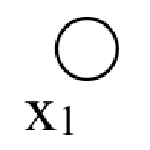
\includegraphics[width=0.08\linewidth]{figures/graphical_models/x1.pdf}}
\caption{A graphical model with only one node.}
\end{figure}

This {\bf graph}
\index{Graph}
is just a single node for the variable $x_1$.  There is no restriction
imposed by the graph on the functional form of its probability function.
In keeping with notation we'll use later, we write that the
probability distribution over $x_1$, $p(x_1) = \phi_1(x_1)$.

Another trivial graphical model is this:
\begin{figure}
\centerline{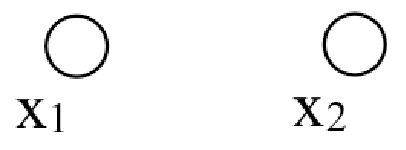
\includegraphics[width=0.2\linewidth]{figures/graphical_models/x1x2.pdf}} 
\caption{Two independent variables.}
\end{figure}

Here, the lack of a
line connecting $x_1$ with $x_2$ indicates a lack of statistical
dependence between these two variables.  In detail, we condition on knowing the
values of any connecting neighbors of $x_1$ and $x_2$ (in this case there
are none) and thus $x_1$ and $x_2$ are statistically independent.  Because of
that independence, the joint probability depicted by this graphical
model must be a product of each variable's marginal probability and thus
must have the form:  $p(x_1, x_2) = \phi_1(x_1) \phi_2(x_2) $.

Let's add a line between these two variables:
\begin{figure}
\centerline{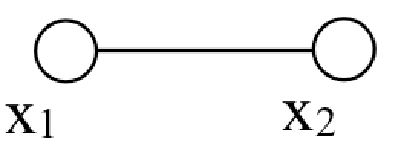
\includegraphics[width=0.16\linewidth]{figures/graphical_models/x1bx2.pdf}} 
\caption{Two dependent variables.}
\end{figure}

By that graph, we
mean that there may be a statistical dependency between
the two variables.  The class of probability
distributions depicted here is now more general than the one above, and we can
only write that the joint probability as some unknown function of
$x_1$ and $x_2$, $p(x_1, x_2) = \phi_{12}(x_1, x_2)$.  This graph
offers no simplification from the most general probability function of
two variables.

Here is a graph with some structure:
\begin{figure}
\centerline{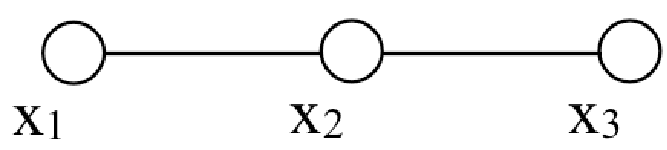
\includegraphics[width=0.24\linewidth]{figures/graphical_models/x1bx2bx3.pdf}} 
\caption{Three dependent variables.}
\label{graph:3node}
\end{figure}

This graph means that if we condition on the variable $x_2$,
then $x_1$ and $x_3$ are independent.  A general form for
$p(x_1, x_2, x_3)$ that guarantees such conditional independence is
\begin{equation}
p(x_1, x_2, x_3) =  \phi_{12}(x_1, x_2)  \phi_{23}(x_2, x_3).
\label{eq:x1x2x3}
\end{equation}
Note the conditional independence implicit in \eqn{\ref{eq:x1x2x3}}:  if the value of $x_2$ is given
(indicated by the solid circle in the graph below), then
the joint probability of \eqn{\ref{eq:x1x2x3}} becomes a product of
some function $f(x_1)$ times some other function $g(x_3)$, revealing
the conditional independence of $x_1$ and $x_3$.  Graphically, we denote the conditioning on the variable $x_2$ with a filled circle for that node:
\begin{figure}
\centerline{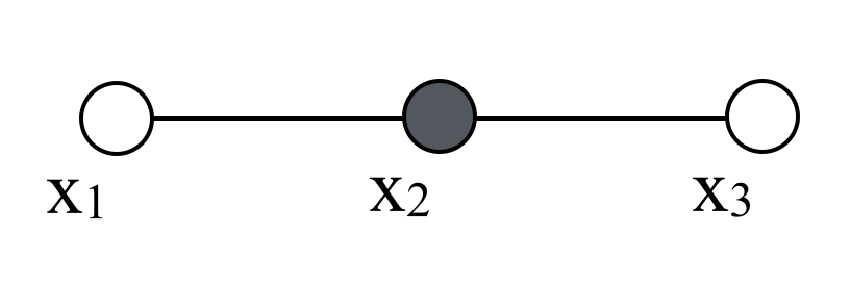
\includegraphics[width=0.26\linewidth]{figures/graphical_models/3node.pdf}} 
\caption{Conditioning on the variable $x_2$ is indicated by the filled circle.}
\label{graph:3node2}
\end{figure}

We will exploit that structure of the joint
probability to perform inference efficiently using an algorithm called belief propagation (BP).

A celebrated theorem, the {\bf Hammersley-Clifford theorem} \cite{Hammersley1971}, tells 
the form the joint probability must have for any given graphical model.
The joint probability for a probabilistic graphical model must be
a product of functions of each the {\bf maximal cliques} 
\index{Maxima cliques}
of the
graph.  Here we define the terms.

A {\bf clique}
\index{Clique}
is any set of nodes where each node is connected to
every other node in the clique.  These graphs illustrate the 
clique property:
\begin{figure}
\centerline{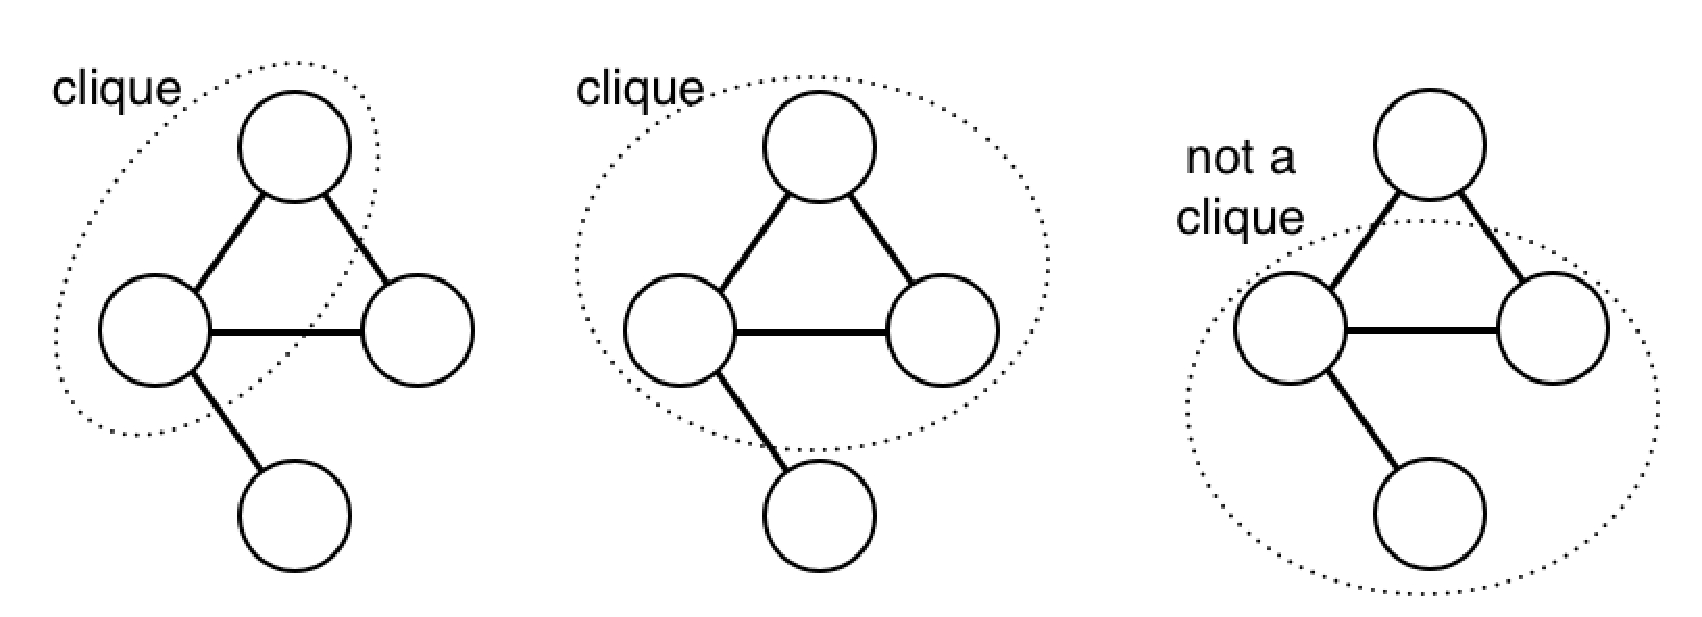
\includegraphics[width=0.5\linewidth]{figures/graphical_models/cliques1.pdf}}
\caption{A clique is any set of nodes where each node is connected to
every other node in the same clique.}
\end{figure}

A {\bf maximal clique}
\index{Maximal clique} is a clique that
can't include more nodes of the graph without losing the clique property.
The sets of nodes below form maximal cliques (left), or do not (right):
\begin{figure}
\centerline{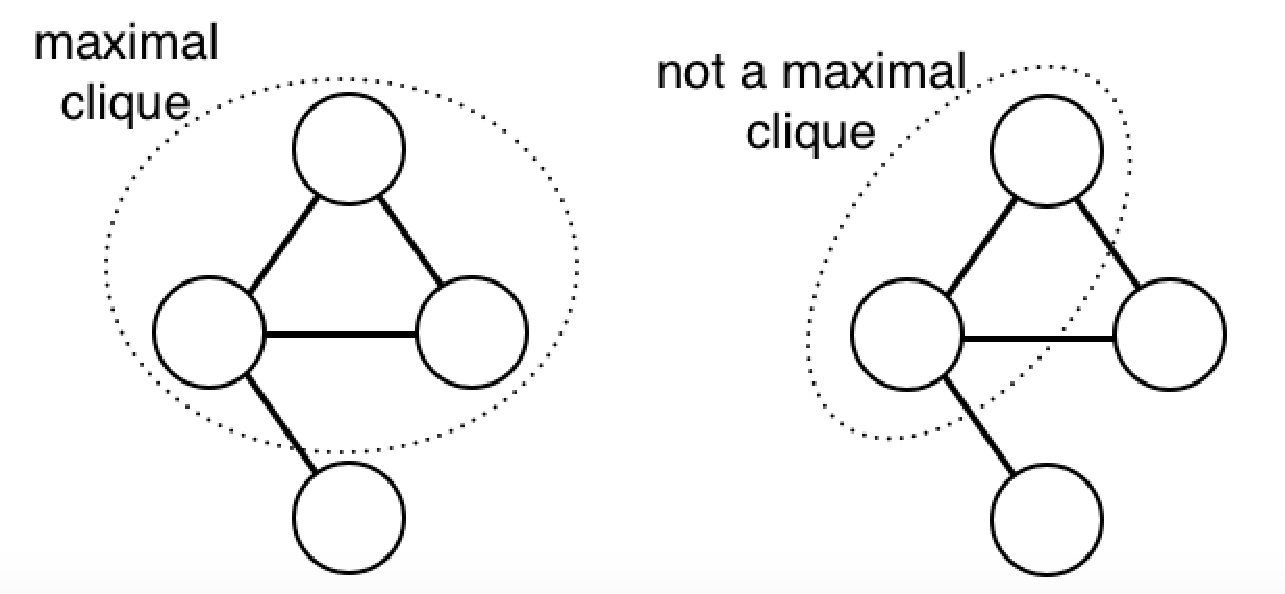
\includegraphics[width=0.4\linewidth]{figures/graphical_models/cliques2.pdf}}
\caption{A maximal clique is the largest possible clique.}
\end{figure}

The {\bf Hammersley-Clifford theorem} \cite{Hammersley1971}
states that a positive probability distribution has the independence structure described by
a graphical model if and only if it can be written as a product of functions
over the variables of each maximal clique:
\begin{equation}
p(x_1, x_2, \ldots, x_N) =  \prod_{x_c  \in x_i} \Psi_{c} (x_c),
\end{equation}
where the product is over all maximal cliques $x_c$ in the graph, $x_i$.

In the example of graph in \fig{\ref{graph:3node}}, the maximal cliques  are (x1,
x2) and (x2, x3), so the Hammersley-Clifford theorem says that the
corresponding joint probability must be of the form of
\eqn{\ref{eq:x1x2x3}}. 

Now we examine some graphical model structures that are especially useful in vision.
In perception problems, we typically have both observed and 
unobserved variables.  The graph below shows a simple {\bf Markov chain} \cite{Gagniuc1989} \index{Markov chain} structure
with three observed variables, shaded, labeled $y_i$, and three
unobserved variables, labeled $x_i$:
\begin{figure}
\centerline{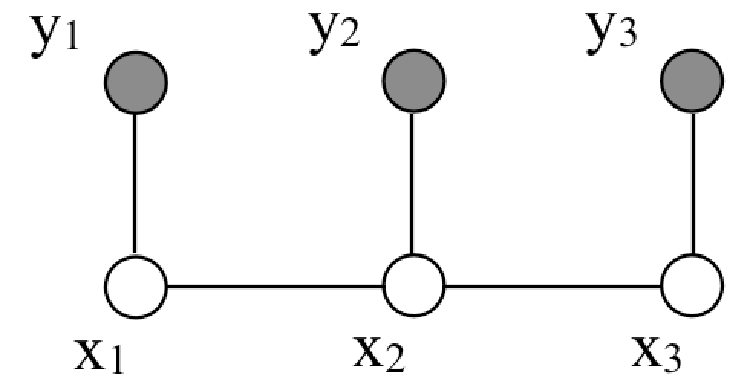
\includegraphics[width=0.36\linewidth]{figures/graphical_models/x1x2x3y1y2y3.pdf}} 
\caption{Markov chain  with three observed variables, shaded, and three unobserved variables.}
\label{fig:chain}
\end{figure}

This is  a chain because
the variables form a linear sequence.  It's a Markov chain structure because the
hidden variables have the Markov property:  conditional on 
 $x_2$, variable $x_3$ is independent of variable $x_1$.  The joint
probability of all the variables shown here is
$p(x_1, x_2, x_3, y_1, y_2, y_3) =  \phi_{12}(x_1, x_2)  \phi_{23}(x_2, x_3)
\psi_{1}(y_1, x_1) \psi_{2}(y_2, x_2) \psi_{3}(y_3, x_3) $.   Using
$p(a,b) = p(a \given b) p(b)$, we can
also write the probability of the $x$ variables conditioned on the
observations $y$,
\begin{equation}
p(x_1, x_2, x_3 \given y_1, y_2, y_3) =  
\frac{1}{p(\mathbf{y})} \phi_{12}(x_1, x_2)  \phi_{23}(x_2, x_3) \psi_{1}(y_1, x_1) \psi_{2}(y_2, x_2) \psi_{3}(y_3, x_3). 
\end{equation}
For brevity, we write $p(\mathbf{y})$ for $p(y_1, y_2, y_3)$.  Thus, to
form the conditional distribution, within a normalization factor, we simply include the observed variable
values into the joint probability.
For vision applications, we often use such Markov chain structures to
describe events over time.  


To capture relationships over space, a two-dimensional (2D)
structure is useful, called a {\bf Markov random field} (MRF) 
\index{Markov random field}
\cite{Blake2011}:
\begin{figure}
\centerline{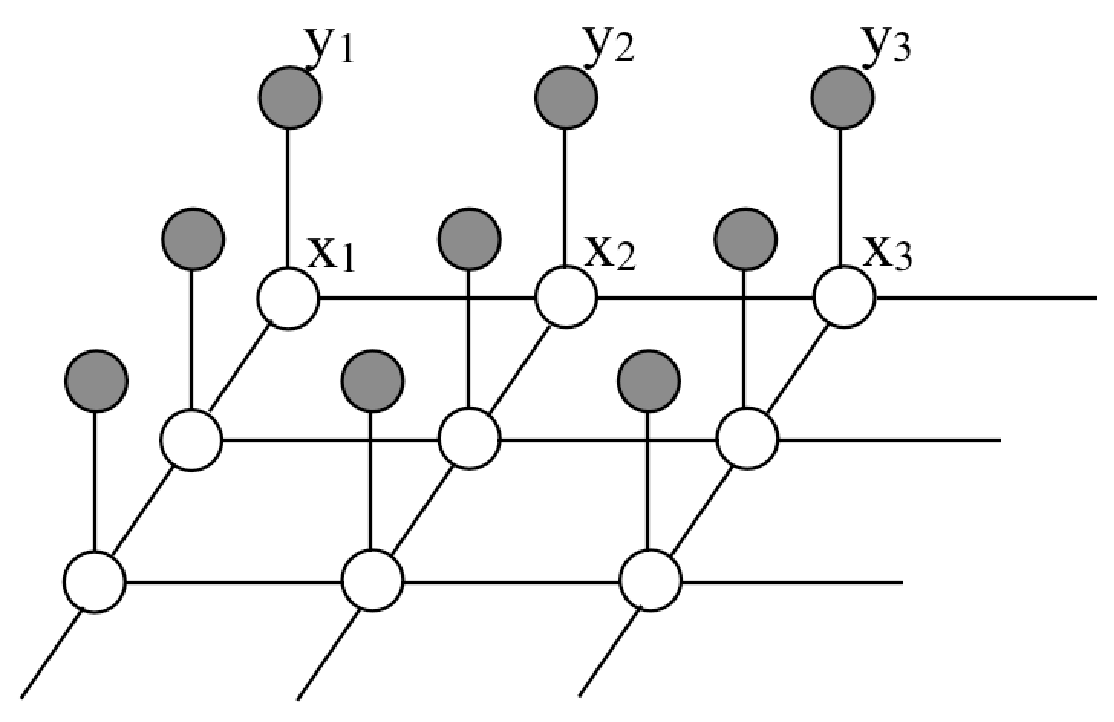
\includegraphics[width=0.48\linewidth]{figures/graphical_models/mrf.pdf}} 
\caption{Two-dimensional Markov random field.}
\end{figure}

Then the joint probability over all the variables factorizes into this product:
\begin{equation}
p(\mathbf{x} \given \mathbf{y}) = 
\frac{1}{p(\mathbf{y})}
\prod_{(i,j)} \phi_{ij}(x_i, x_j) \prod_i \psi_i(x_i, y_i),
\end{equation}
where the first product is over all spatial neighbors $i$
and $j$, and the second product is over all nodes $i$.

\begin{comment}
\begin{figure}
\centerline{
\sublabel{a}{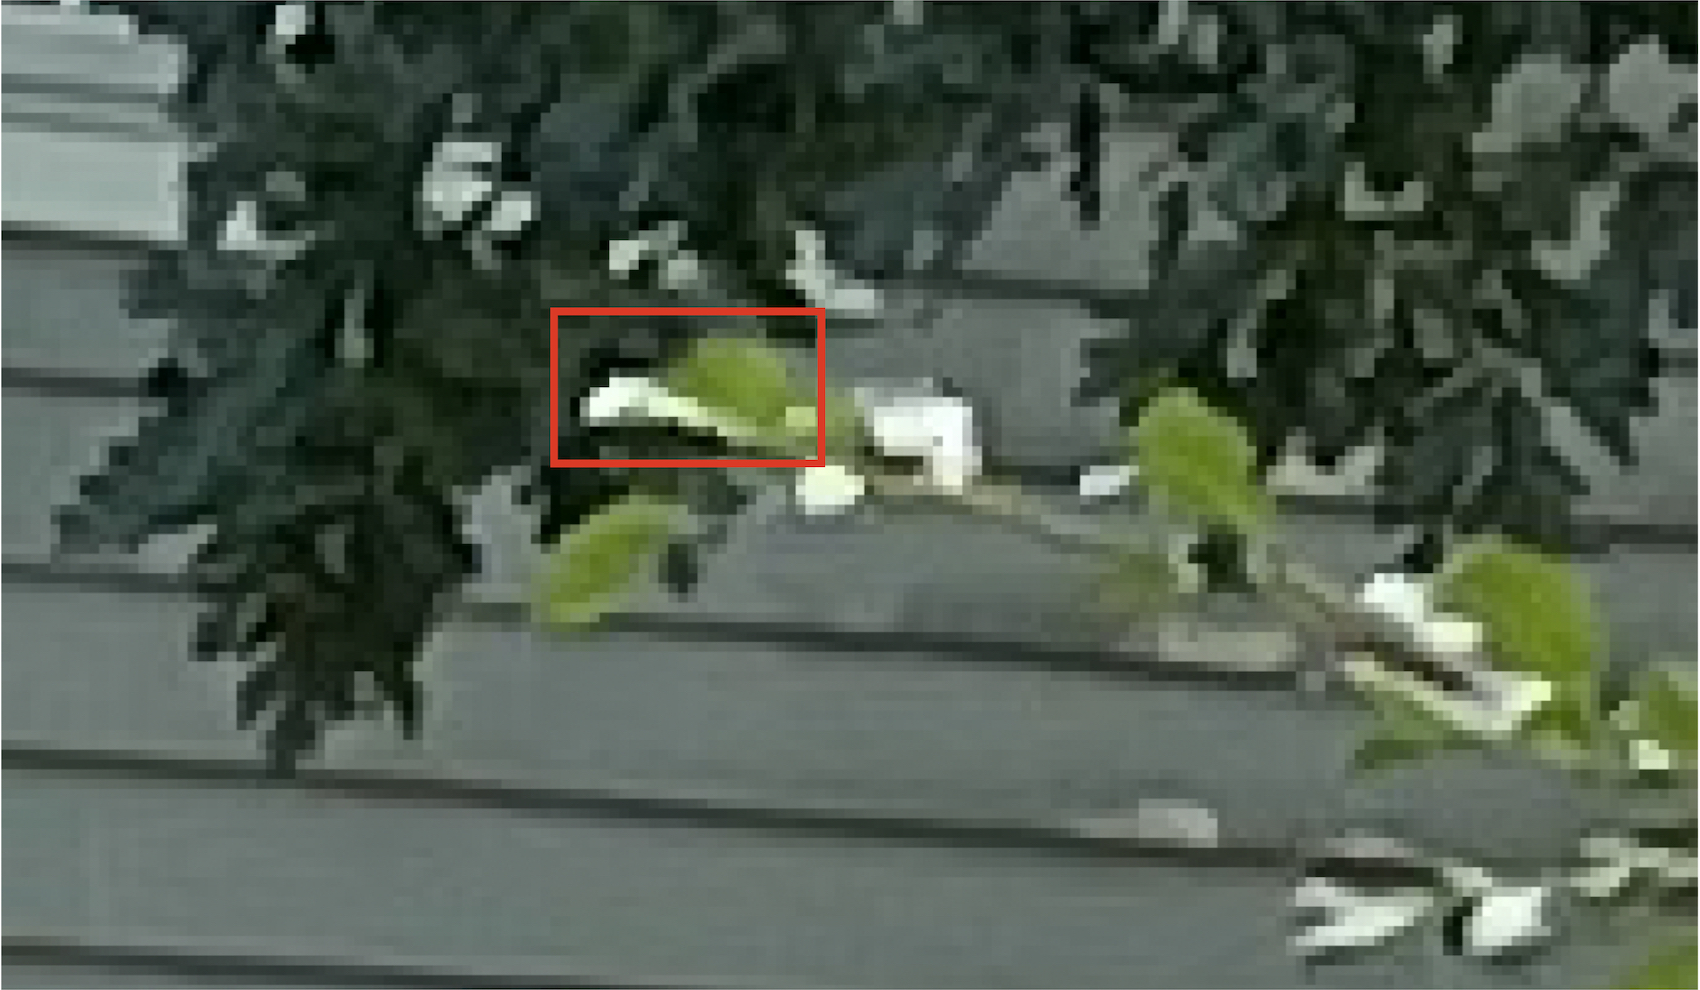
\epsfig{file=figures/graphical_models/leaf2.jpg,width=2.2in}}
\sublabel{b}{
\epsfig{file=figures/graphical_models/leaf3.jpg,width=2.2in}}}
%\sublabel{c}{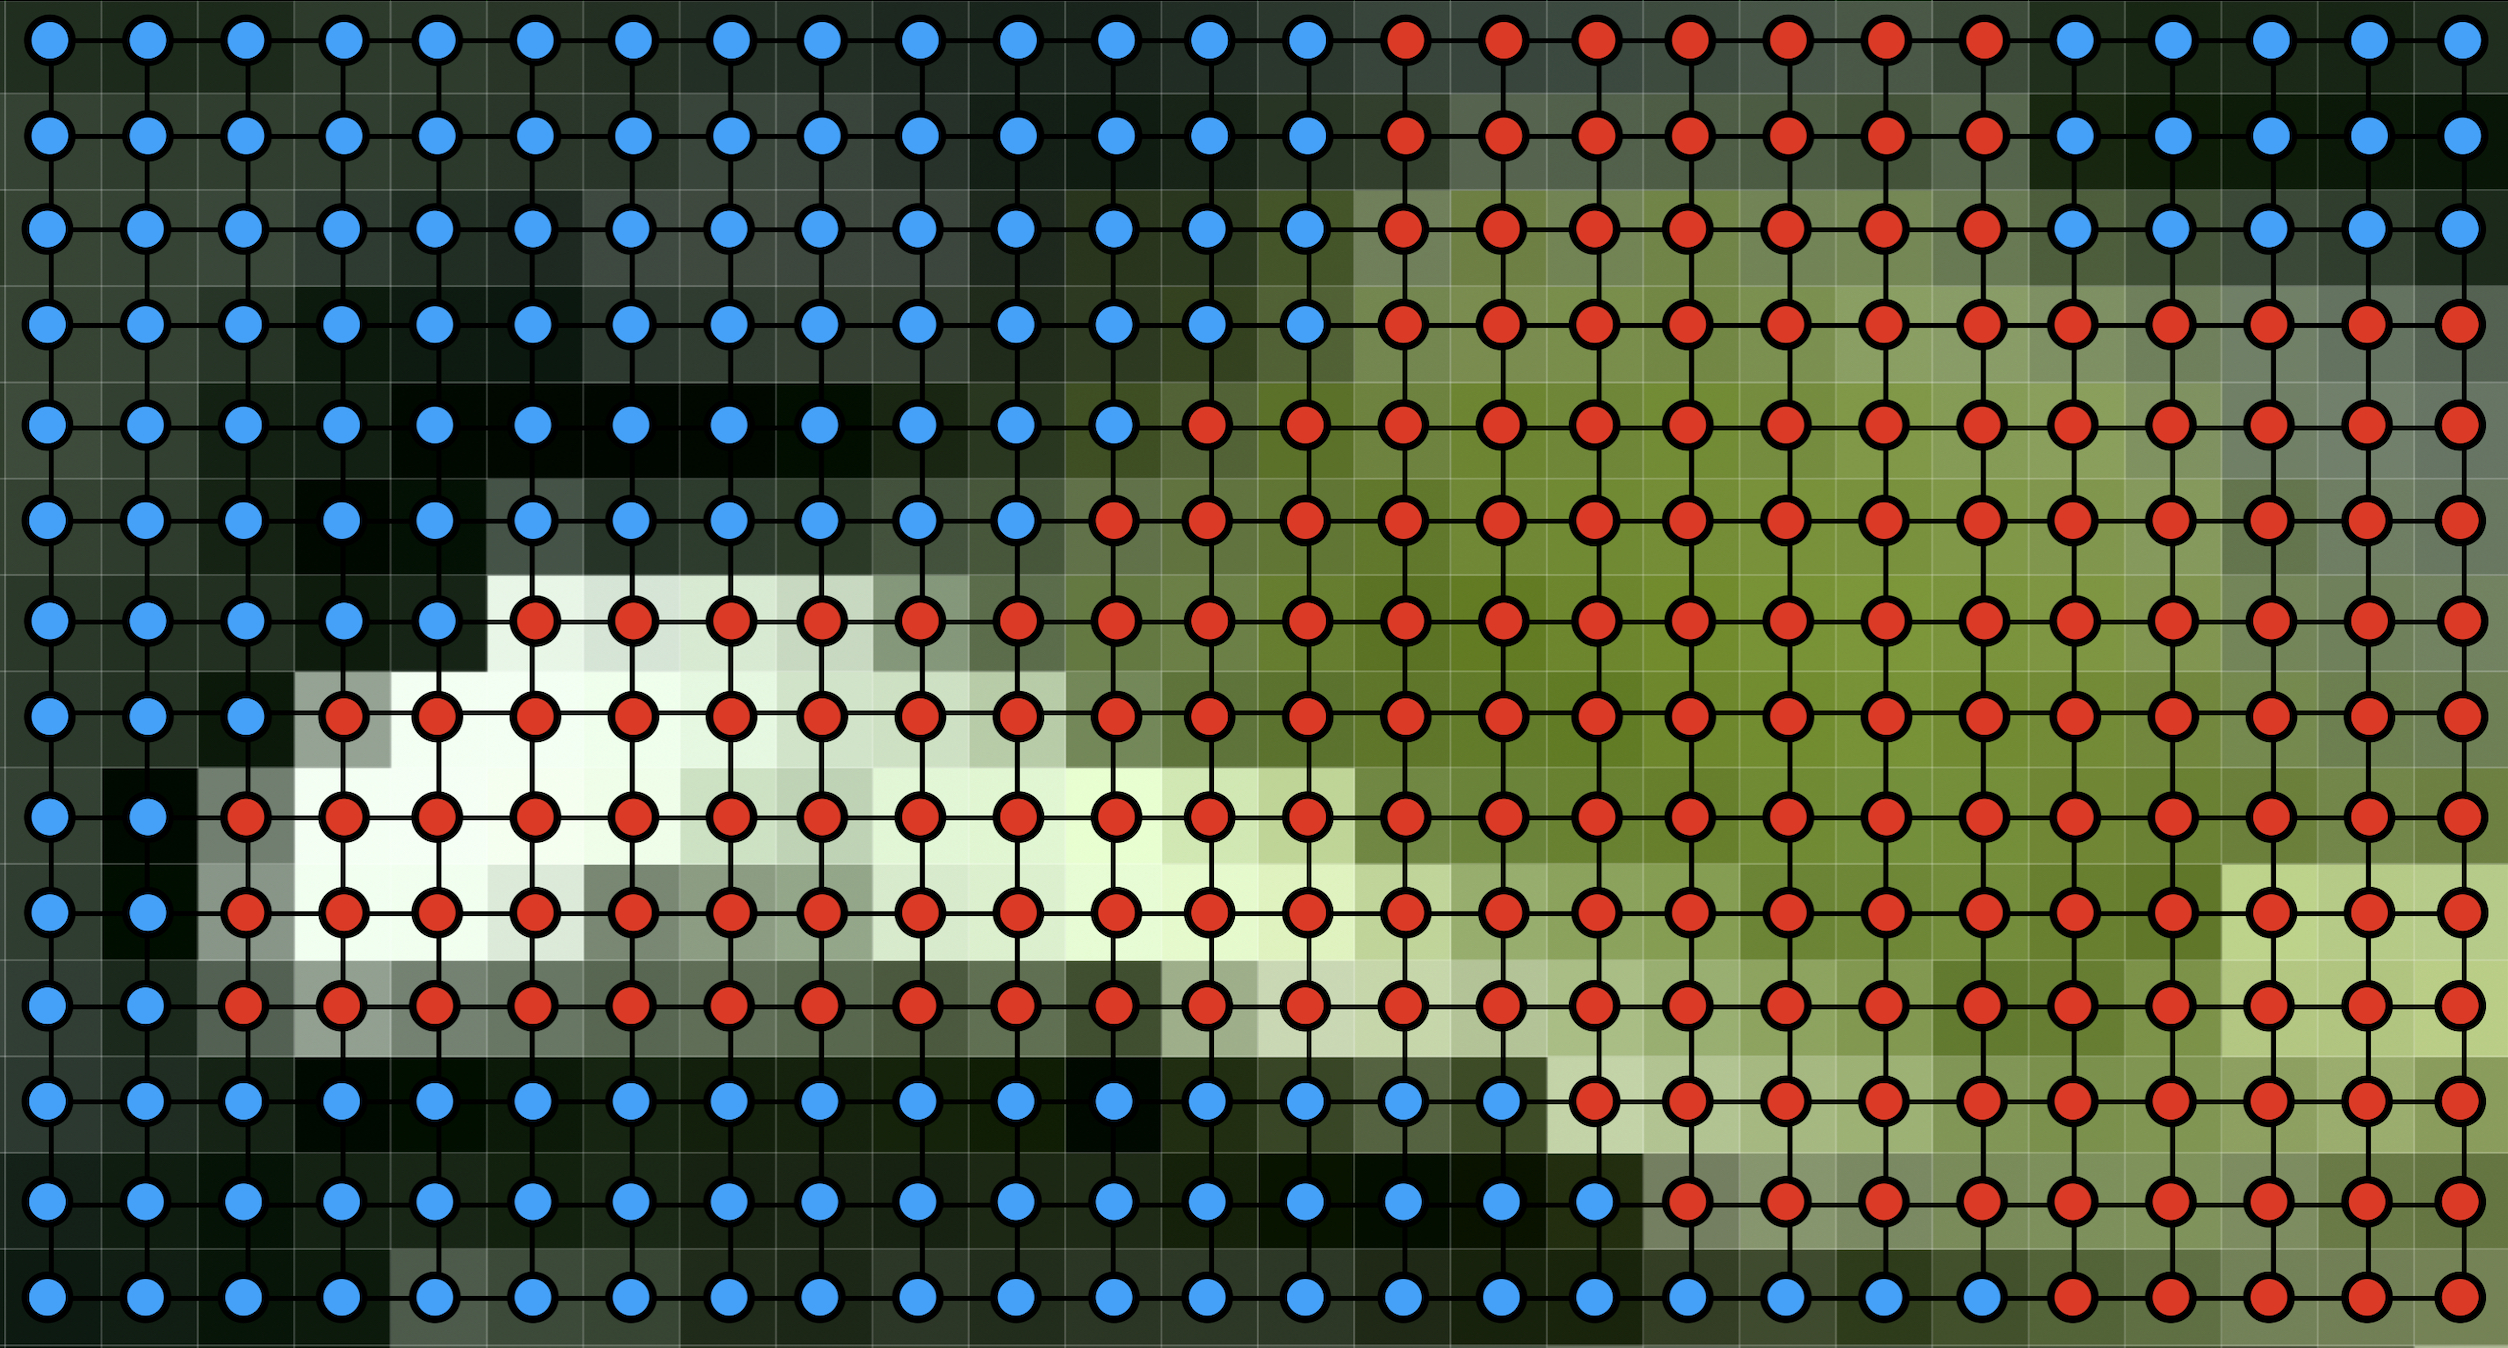
\epsfig{file=figures/graphical_models/leaf1,width=1.4in}}}
\centerline{
%\hspace{1in}
\sublabel{c}{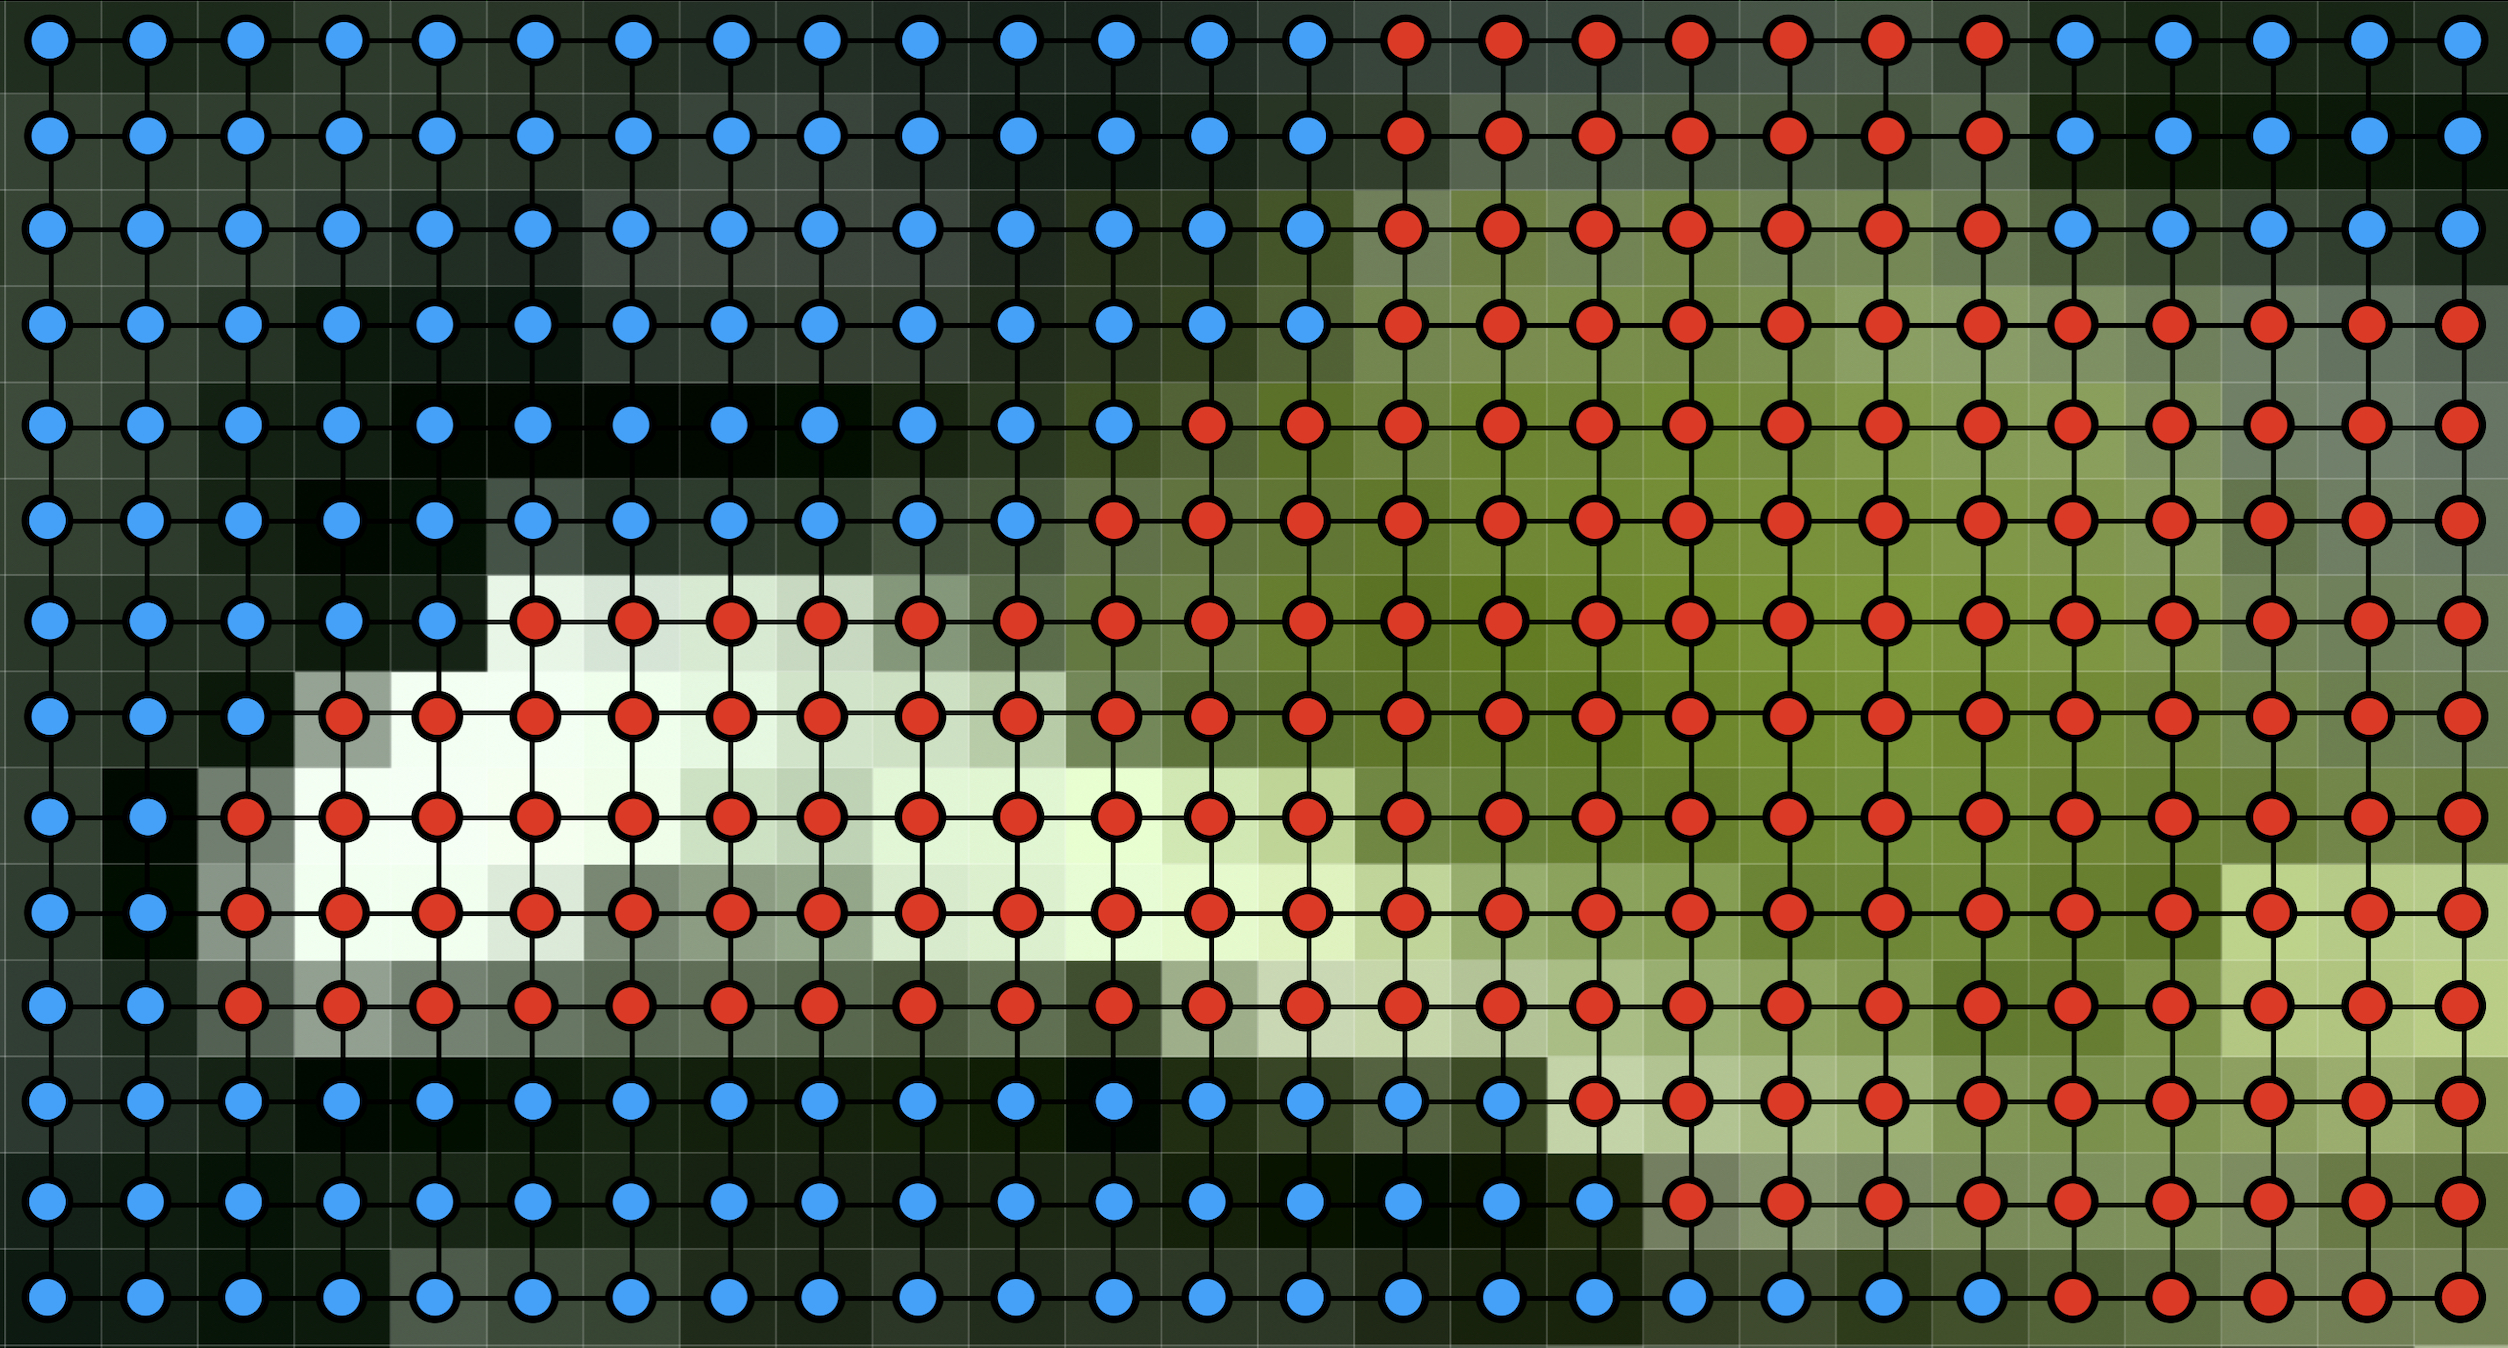
\epsfig{file=figures/graphical_models/leaf1,width=4.4in}}}
\caption{(a) Image to be segmented. (b) A local region of (a).  (c) Visualization of an MRF of nodes corresponding to image pixels, with states indicating segment membership, for a hypothetical most probable configuration.}
\label{fig:leafs}
\end{figure}
\end{comment}



An example of how Markov random field models are applied to images is depicted in \fig{\ref{fig:leafs}}, which show a small image region and its context in the image (\fig{\ref{fig:leafs}}[a]). \Fig{\ref{fig:leafs}}(b) shows an MRF with each node corresponding to a pixel of the image region.  The states of an MRF can be indicator variables of image segment membership for each pixel. The states of a hypothetical most-probable configuration of this MRF are shown as the color of each node in this illustration.


\begin{figure}
\centerline{
\sublabel{a}{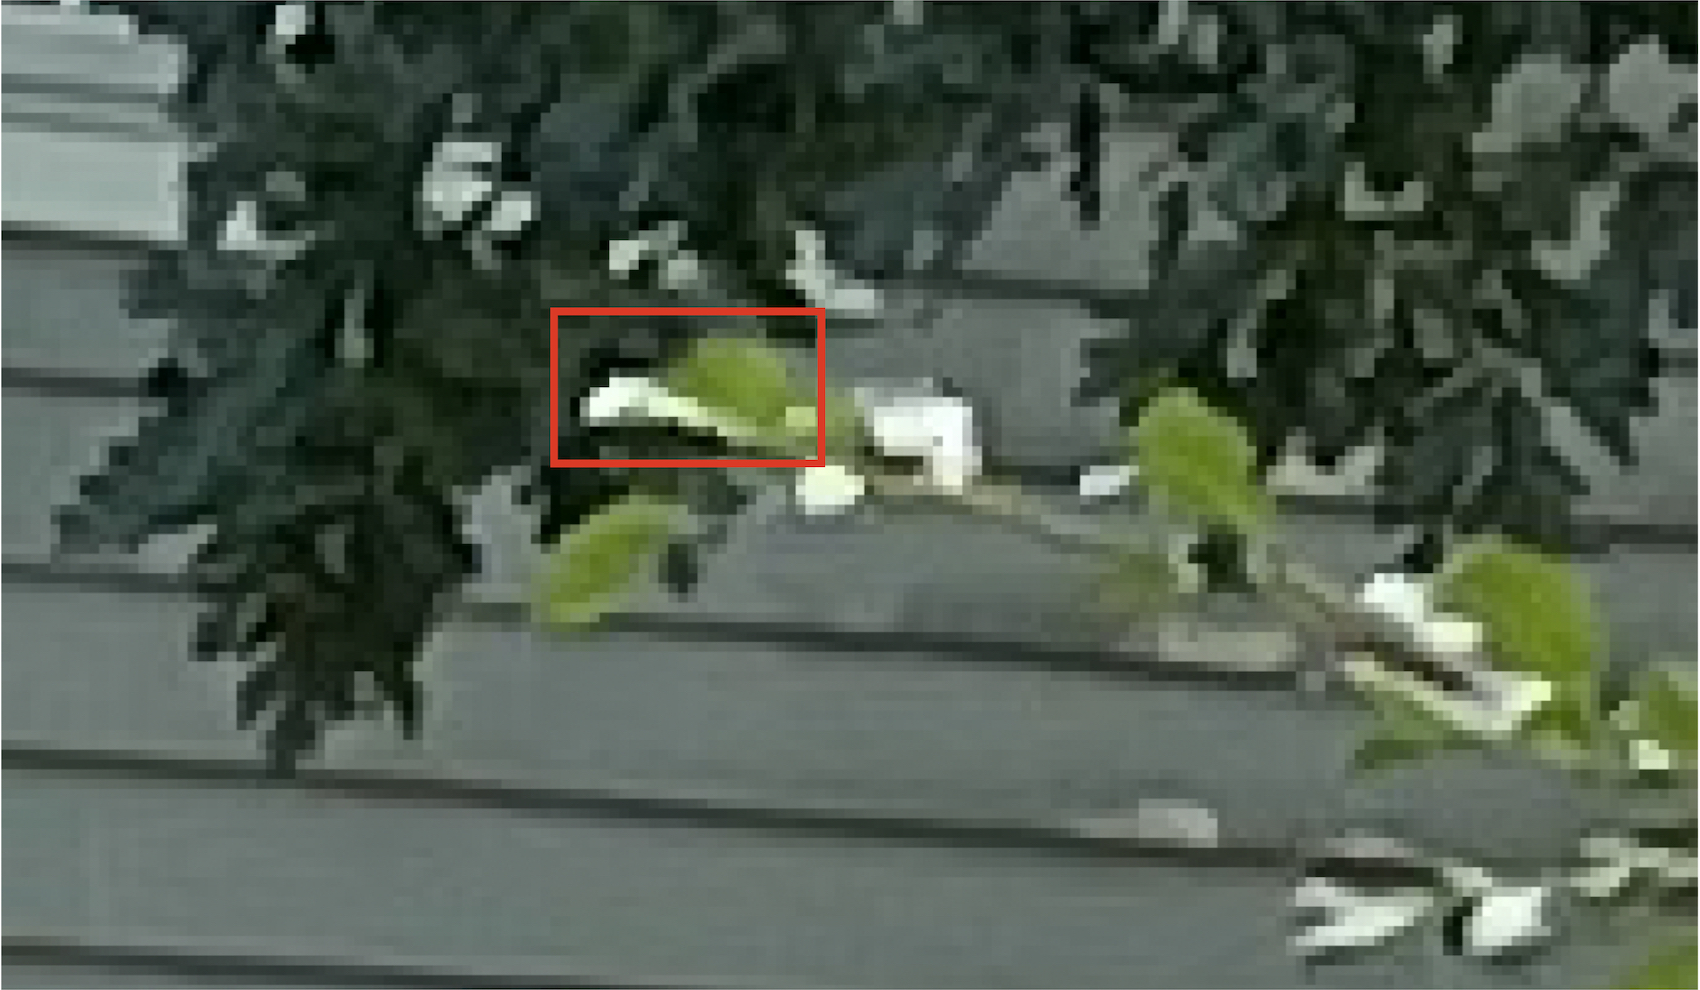
\epsfig{file=figures/graphical_models/leaf2.jpg,width=2.3in}}
\sublabel{b}{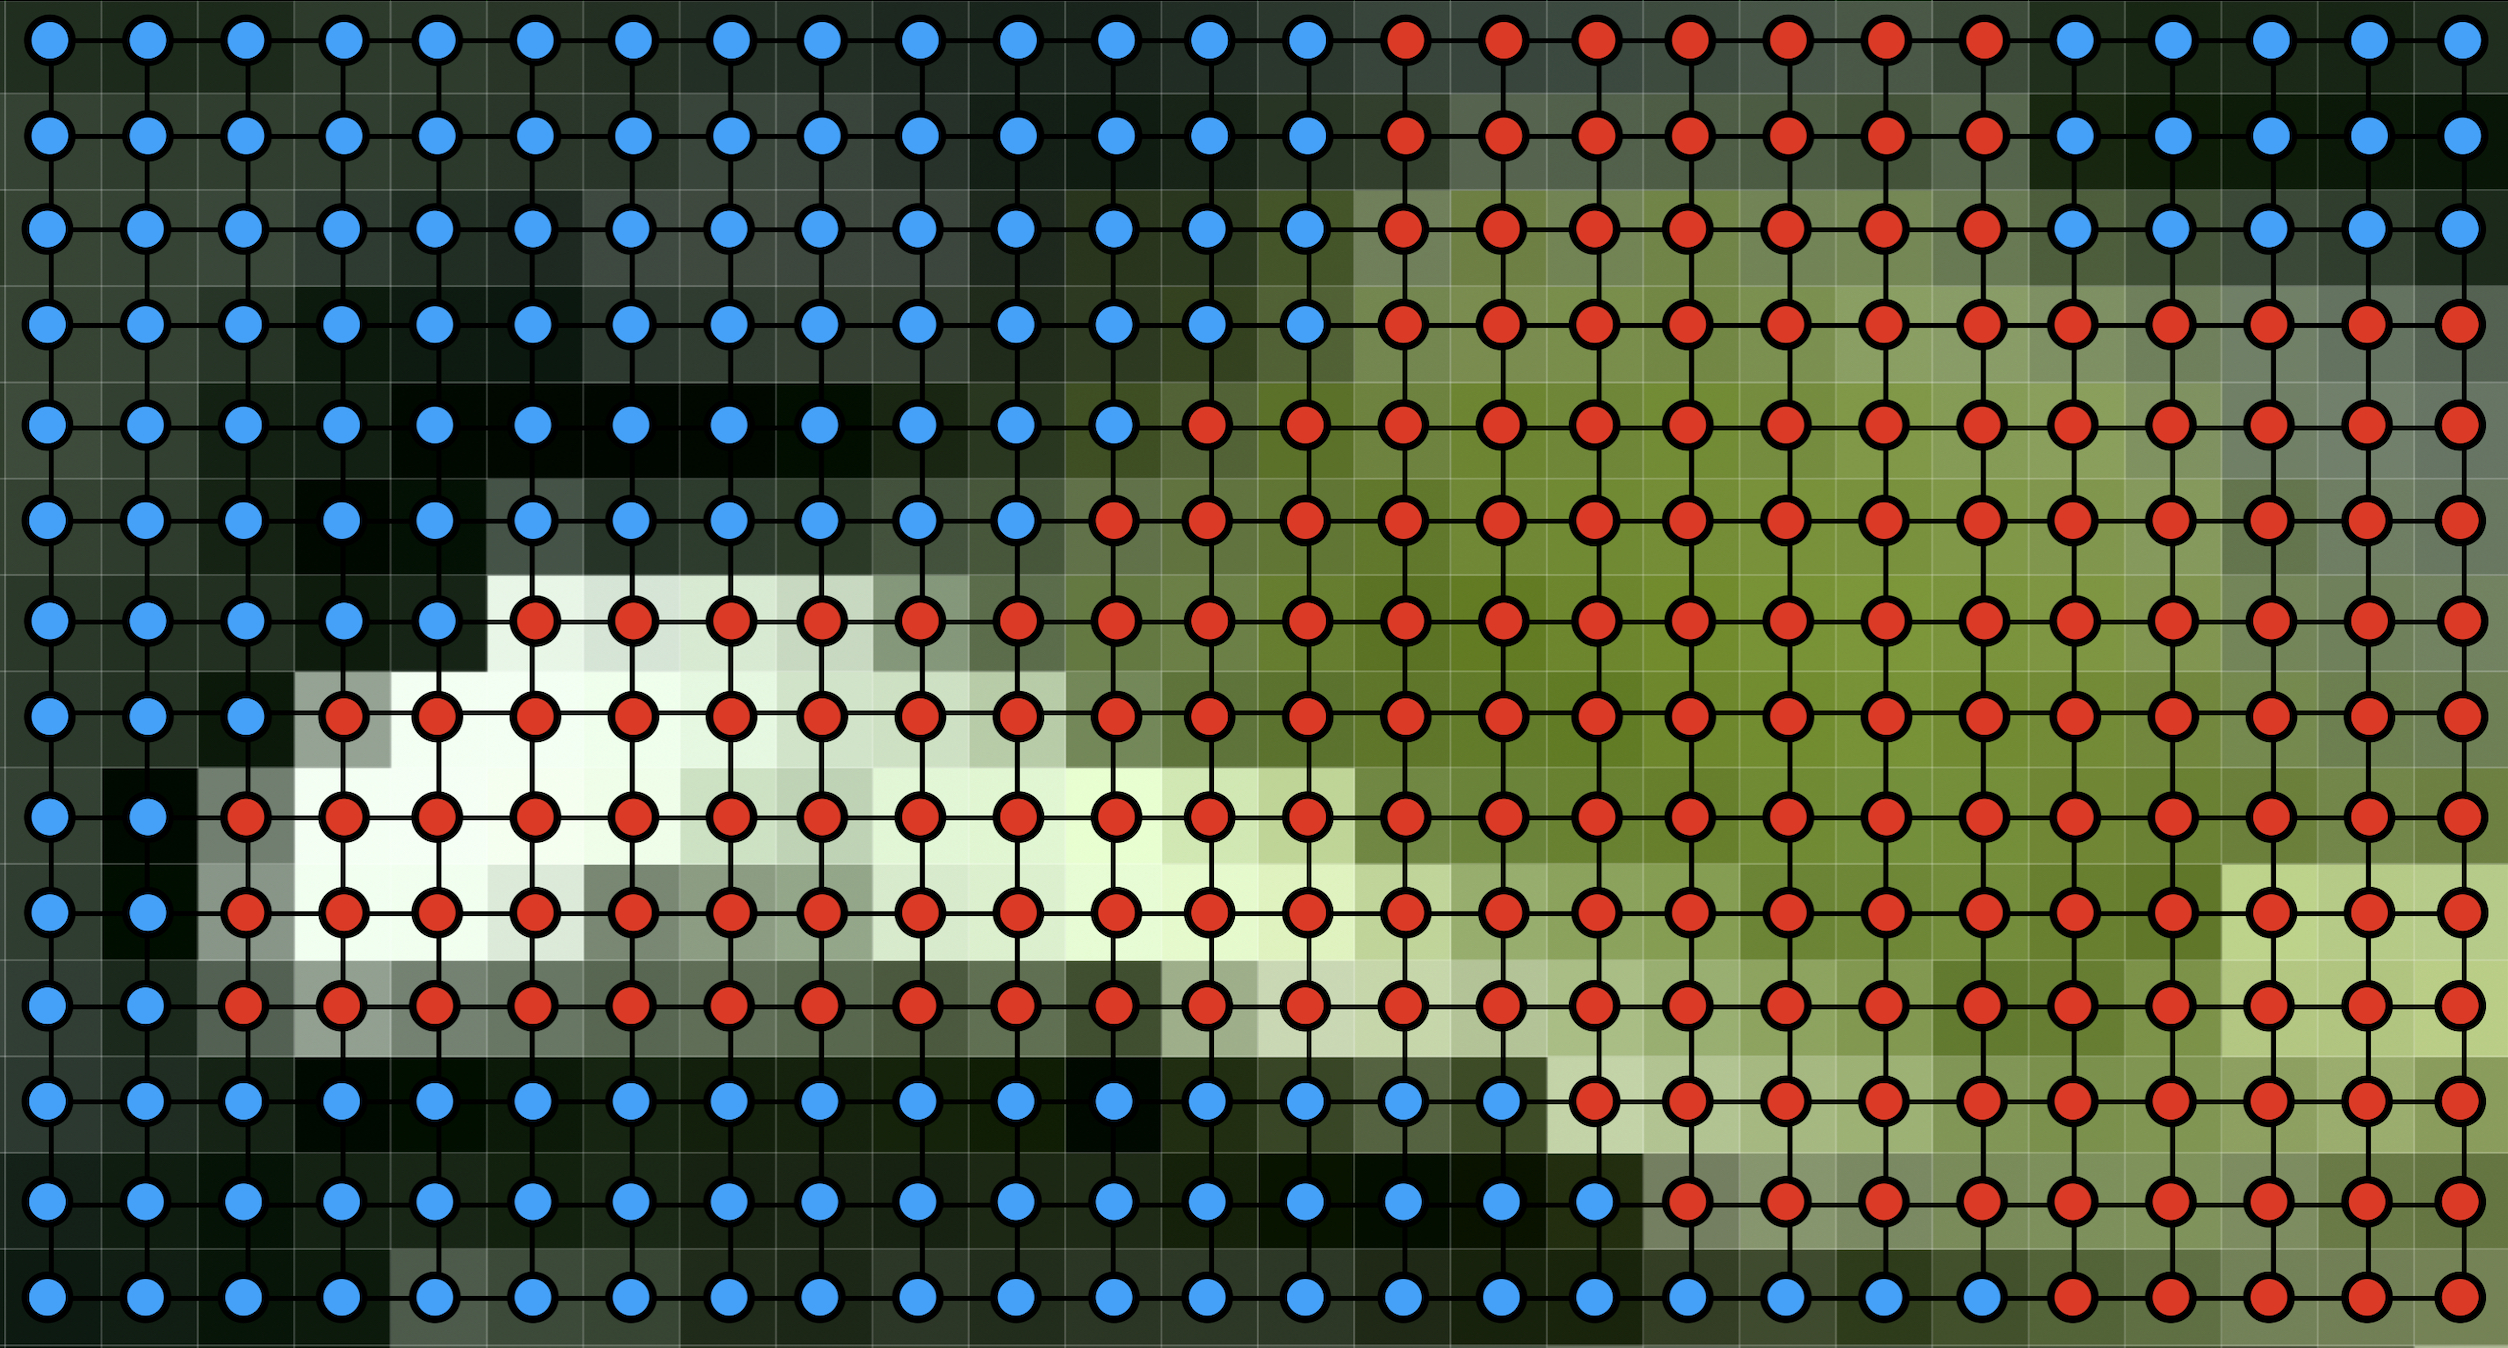
\epsfig{file=figures/graphical_models/leaf1,width=2.5in}}}
\caption{(a) Image to be segmented and a local region of (a) marked in red.  (b) Visualization of an MRF of nodes corresponding to image pixels inside the marked region, with states indicating segment membership, for a hypothetical most probable configuration.}
\label{fig:leafs}
\end{figure}

%\clearpage

\section{Directed Graphical Models}


In addition to undirected graphical models, another
type of graphical  model is commonly used.
{\bf Directed graphical models} \cite{Koller2009} describe factorizations of the joint
probability into products of conditional probability distributions.  
Each node in a directed graph contributes a
well-specified factor in the joint probability:  the probability of
its variable, conditioned all the variables originating arrows
pointing into it.  So this graph
\begin{figure}
\centerline{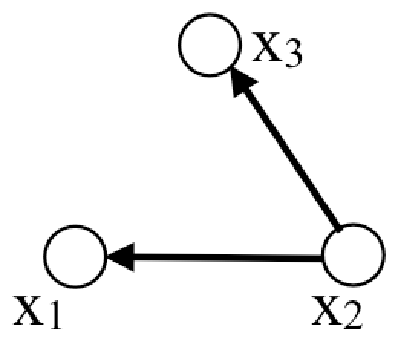
\includegraphics[width=0.20\linewidth]{figures/graphical_models/directed.pdf}} 
\caption{A directed graphical model with three variables.}
\end{figure}

\noindent denotes the joint probability, 
\begin{equation}
p(x_1, x_2, x_3) = p(x_2)  p(x_1 \given x_2) p(x_3 \given x_2) 
\label{eq:directedjoint}
\end{equation}

The general rule for writing the joint probability described by a
directed graph is this:  Each node, $x_n$, contributes the factor
$p(x_n \given x_{\Xi})$, where $\Xi$ is the set of nodes with arrows pointing
in to node $x_n$.  You can verify that \eqn{\ref{eq:directedjoint}}
follows this rule.  Directed graphical models are often used to describe causal processes.

\section{Inference in Graphical Models}

Given a probabilistic graphical model and observations, we want to estimate the states of 
the unobserved variables. For example, given image
observations, we may want to estimate the pose of the person.
The {\bf belief propagation} algorithm lets us do that efficiently.

\index{Bayes' theorem}
Recall the Bayesian inference task:  our observations are the
elements of a vector, $\mathbf{y}$, and we seek to infer the probability
$p(\mathbf{x} \given \mathbf{y})$ of some scene
parameters, $\mathbf{x}$, given the observations. 
By Bayes' theorem, we have
\begin{equation}
p(\mathbf{x} \given \mathbf{y}) = \frac{p(\mathbf{y} \given \mathbf{x}) p(\mathbf{x}) }{p(\mathbf{y}) }
\end{equation}
The {\bf likelihood term} 
\index{Likelihood}
$p(\mathbf{y} \given \mathbf{x})$ describes how a
rendered scene $\mathbf{x}$ generates observations $\mathbf{y}$.  The {\bf
prior probability}, 
\index{Prior probability}
$p(\mathbf{x})$, tells the probability of any given
scene $\mathbf{x}$ occurring.  For inference, we often ignore the denominator,
$P(\mathbf{y})$, called the {\bf evidence}, as it is constant with
respect to the variables we seek to estimate, $\mathbf{x}$.

\marginnote{The statistician Harold Jeffreys wrote, "Bayes' theorem is to the theory of probability what Pythagorus' theorem is to geometry" \cite{Jeffreys1973}}

Typically, we make many observations, $\mathbf{y}$, of the variables of some system,
and we want to find the the state of some hidden variable, $\mathbf{x}$, given those
observations.  The posterior probability, $p(\mathbf{x} \given \mathbf{y})$, tells
us the probability for any value of the hidden variables, $\mathbf{x}$.
From this posterior probability, we often want some single {\em best} estimate for $\mathbf{x}$,
denoted $\mathbf{\hat{x}}$ and called a point estimate.  

Selecting the best estimate $\mathbf{\hat{x}}$ requires specifying a
penalty for making a wrong guess. If we penalize all wrong answers
equally, the best strategy is to guess the value of  $\mathbf{x}$ that maximizes
the posterior probability, $p(\mathbf{x} \given \mathbf{y})$ (because any other
explanation $\mathbf{\hat{x}}$ for the observations $\mathbf{y}$  would be
less probable).  That is called the {\bf maximum a posteriori} (MAP) estimate.
\index{Maximum a posteriori}

But we may want to penalize wrong answers as a function of how far
they are from the correct answer.  If that penalty function is
the squared distance in $\mathbf{x}$, then the point estimate that
minimizes the average value of that error is called the {\bf minimum mean squared error}
estimate (MMSE).
\index{Minimum mean squared error}
To find this estimate, we seek 
the $\hat{\mathbf{x}}$ that minimizes the squared error, weighted by the probability of each outcome:
\begin{equation}
\hat{\mathbf{x}}_{MMSE} = \mbox{argmin}_{\tilde{\mathbf{x}}} 
\int_{\mathbf{x}} p(\mathbf{x} \given \mathbf{y}) (\mathbf{x}-\tilde{\mathbf{x}})'
(\mathbf{x}-\tilde{\mathbf{x}}) d\mathbf{x}
\end{equation} 
Differentiating with respect to $\mathbf{x}$ to solve for the stationary
point, the global minimum for this convex function, we find
\begin{equation}
\hat{\mathbf{x}}_{MMSE} = \int_{\mathbf{x}} \mathbf{x} p(\mathbf{x} \given \mathbf{y})  d\mathbf{x}.
\end{equation}
Thus, the minimum mean square error estimate, $\hat{\mathbf{x}}_{MMSE}$,
is the mean of the posterior distribution.  
If $\mathbf{x}$ represents a discretized space, then the
marginalization integrals over $d\mathbf{x}$ become sums over the
corresponding discrete states of $\mathbf{x}$.

\marginnote{For a Gaussian probability distribution, the MAP estimate and the MMSE estimate
are always the same, since the mean of the distribution is always its maximum value.}

For now, we'll assume we seek the MMSE estimate. By the properties of
the multivariate mean, to find the mean at each variable, or node, in
a network, we can first find the marginal probability at each node,
then compute the mean of each marginal probability.  In other words,
given $p(\mathbf{x} \given \mathbf{y})$, we will compute $p(x_i \given \mathbf{y})$,
where $i$ is the $i$-th hidden node.  From $p(x_i \given \mathbf{y})$ it is
simple to compute the posterior mean at node $i$.

For the case of discrete variables, we compute the marginal probability at a node by summing over the states at all the other nodes,
\begin{equation}
    p(x_i \given \mathbf{y}) =  \sum_{j  \mbox{\textbackslash} i} \sum_{x_j} 
    p(x_1, x_2, \ldots, x_i, \ldots, x_N \given \mathbf{y}),
    \label{eq:discreteMarginalization}
\end{equation}
where the notation $j \mbox{\textbackslash} i$ means ``all possible values of $j$ except for $j = i$.''

\section{Simple Example of Inference in a Graphical Model}
\label{sect:simpleexample}

To gain intuition, let's calculate the marginal probability for a
simple example.  Consider the three-node Markov chain 
of \fig{\ref{fig:chain2}}.
\begin{figure}
\centerline{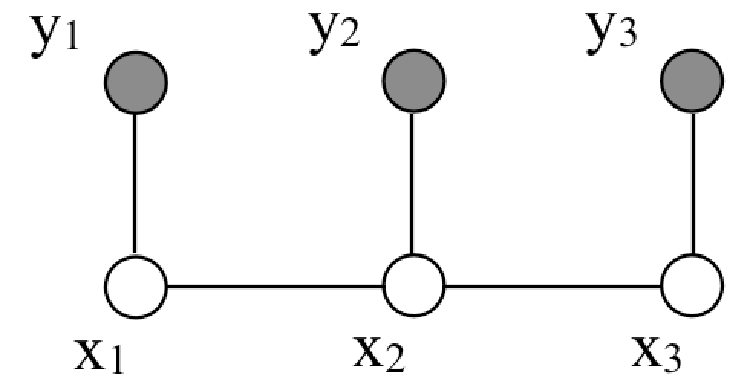
\includegraphics[width=0.36\linewidth]{figures/graphical_models/x1x2x3y1y2y3.pdf}} 
\caption{Same three-node Markov chain of \fig{\ref{fig:chain}}.}
\label{fig:chain2}
\end{figure}

Vision tasks this can apply to include modeling the probability of a pixel
belonging to an object edge, given the evidence, observations $\mathbf{y}$, at a point and two
neighboring locations.  The inferred states $\mathbf{x}$ could be a label
indicating the presence of an edge.

We seek to marginalize the joint probability in order to
find the marginal probability at node 1, $p(x_1 \given \mathbf{y})$, given
observations $y_1$, $y_2$, and $y_3$, which we denote as $\mathbf{y}$.
We have, assuming the nodes have discrete states,
\begin{equation}
p(x_1 \given \mathbf{y}) = \sum_{x_2} \sum_{x_3}  p(x_1, x_2, x_3 \given \mathbf{y})
\label{eq:3chain}
\end{equation}

Here's the main point.  If we knew nothing about the structure of
the joint probability $p(x_1, x_2, x_3 \given \mathbf{y})$, the computation would require
$\left| x \right|^3$ computations: a double-sum over all $x_2$ and $x_3$ states must
be computed
for each possible $x_1$ state (we're denoting the number of states of any of the $x$
variables as $\left| x \right|$).  In the more general case, for a Markov chain of
$N$ nodes, we would need $\left| x \right|^N$ summations to compute the desired
marginal at any node of the chain.  Such a computation quickly
becomes intractable as $N$ grows.

But we can exploit the model's structure to avoid the
exponential growth of the computation with $N$.
Substituting the joint probability, from the graphical model, into the
marginalization equation, \eqn{\ref{eq:3chain}}, gives
\begin{equation}
p(x_1 \given \mathbf{y}) = 
\frac{1}{p(\mathbf{y})} \sum_{x_2} \sum_{x_3}  
\phi_{12}(x_1, x_2)  \phi_{23}(x_2, x_3) \psi_{1}(y_1, x_1) \psi_{2}(y_2, x_2) \psi_{3}(y_3, x_3) 
\label{eq:3chainb}
\end{equation}
This form for the joint probability reveals that not every variable is
coupled to every other one.  We can pass summations
through  variables they don't sum over, letting us compute the
marginalization much more efficiently.  This will make only a small
difference for this short chain, but it makes a huge difference
for longer ones.  So we write
\begin{eqnarray}
p(x_1 \given \mathbf{y}) 
& = & 
\frac{1}{p(\mathbf{y})} \sum_{x_2} \sum_{x_3}  
\phi_{12}(x_1, x_2)  \phi_{23}(x_2, x_3)
\psi_{1}(y_1, x_1) \psi_{2}(y_2, x_2) \psi_{3}(y_3, x_3)  
\label{eq:before}
\\
& = &
\frac{1}{p(\mathbf{y})}
\psi_{1}(y_1, x_1) 
\sum_{x_2} \phi_{12}(x_1, x_2) \psi_{2}(y_2, x_2) 
\sum_{x_3}   \phi_{23}(x_2, x_3)  \psi_{3}(y_3, x_3)  
\label{eq:after} 
\end{eqnarray}
That factorization of \eqn{\ref{eq:after}} is the key step.
It reduces the number of terms summed from order $\left| x \right| ^3$ to order $2
\left| x \right|^2$ for this chain, and for a chain of length $N$ chain, from order $\left|x \right|^N$ to order $(N-1) \left|x \right|^2$--from exponential to linear dependence on $N$--a
huge computational savings for large $N$.  

The partial sums of \eqn{\ref{eq:after}} are named  {\bf messages} 
\index{Message}
because they pass information from one node to another.  We call the message from node 3
to node 2, $m_{32}(x_2)  = \sum_{x_3}   \phi_{23}(x_2, x_3)
m_{63}(x_3) $.  The other partial sum is the message from node 2 to
node 1, 
$m_{21}(x_1)   = \sum_{x_2} \phi_{12}(x_1, x_2)  m_{52}(x_2)  
m_{32}(x_2) $.
Note that the messages are always messages about
the states of the node that the message is being sent to, that is, the
arguments of the message $m_{ij}$ are the states $x_j$ of node $j$.  The algorithm corresponding to \eqn{\ref{eq:after}} is called {\bf belief propagation}.

\Eqn{\ref{eq:after}} gives us the marginal probability at node 1.  To
find the marginal probability at another node, we 
can write out the sums over variables needed for that node, pass the
sums through factors in the joint probability that they don't operate
on, to come up with an efficient reorganization of summations analogous to
\eqn{\ref{eq:after}}.  We would find that many
of the summations from marginalization at the node $x_1$  would need
to be recomputed for the marginalization at node $x_2$.  That
motivates storing and reusing the messages, which the belief propagation algorithm does in an optimal way.

\section{Belief Propagation}

For more complicated graphical models, we want to 
replace the manual factorization above
with an automatic procedure for identifying the
computations needed for marginalizations and to 
cache them efficiently.  BP does that by
identifying those reusable sums, that is, the messages. 

\begin{figure}
\centerline{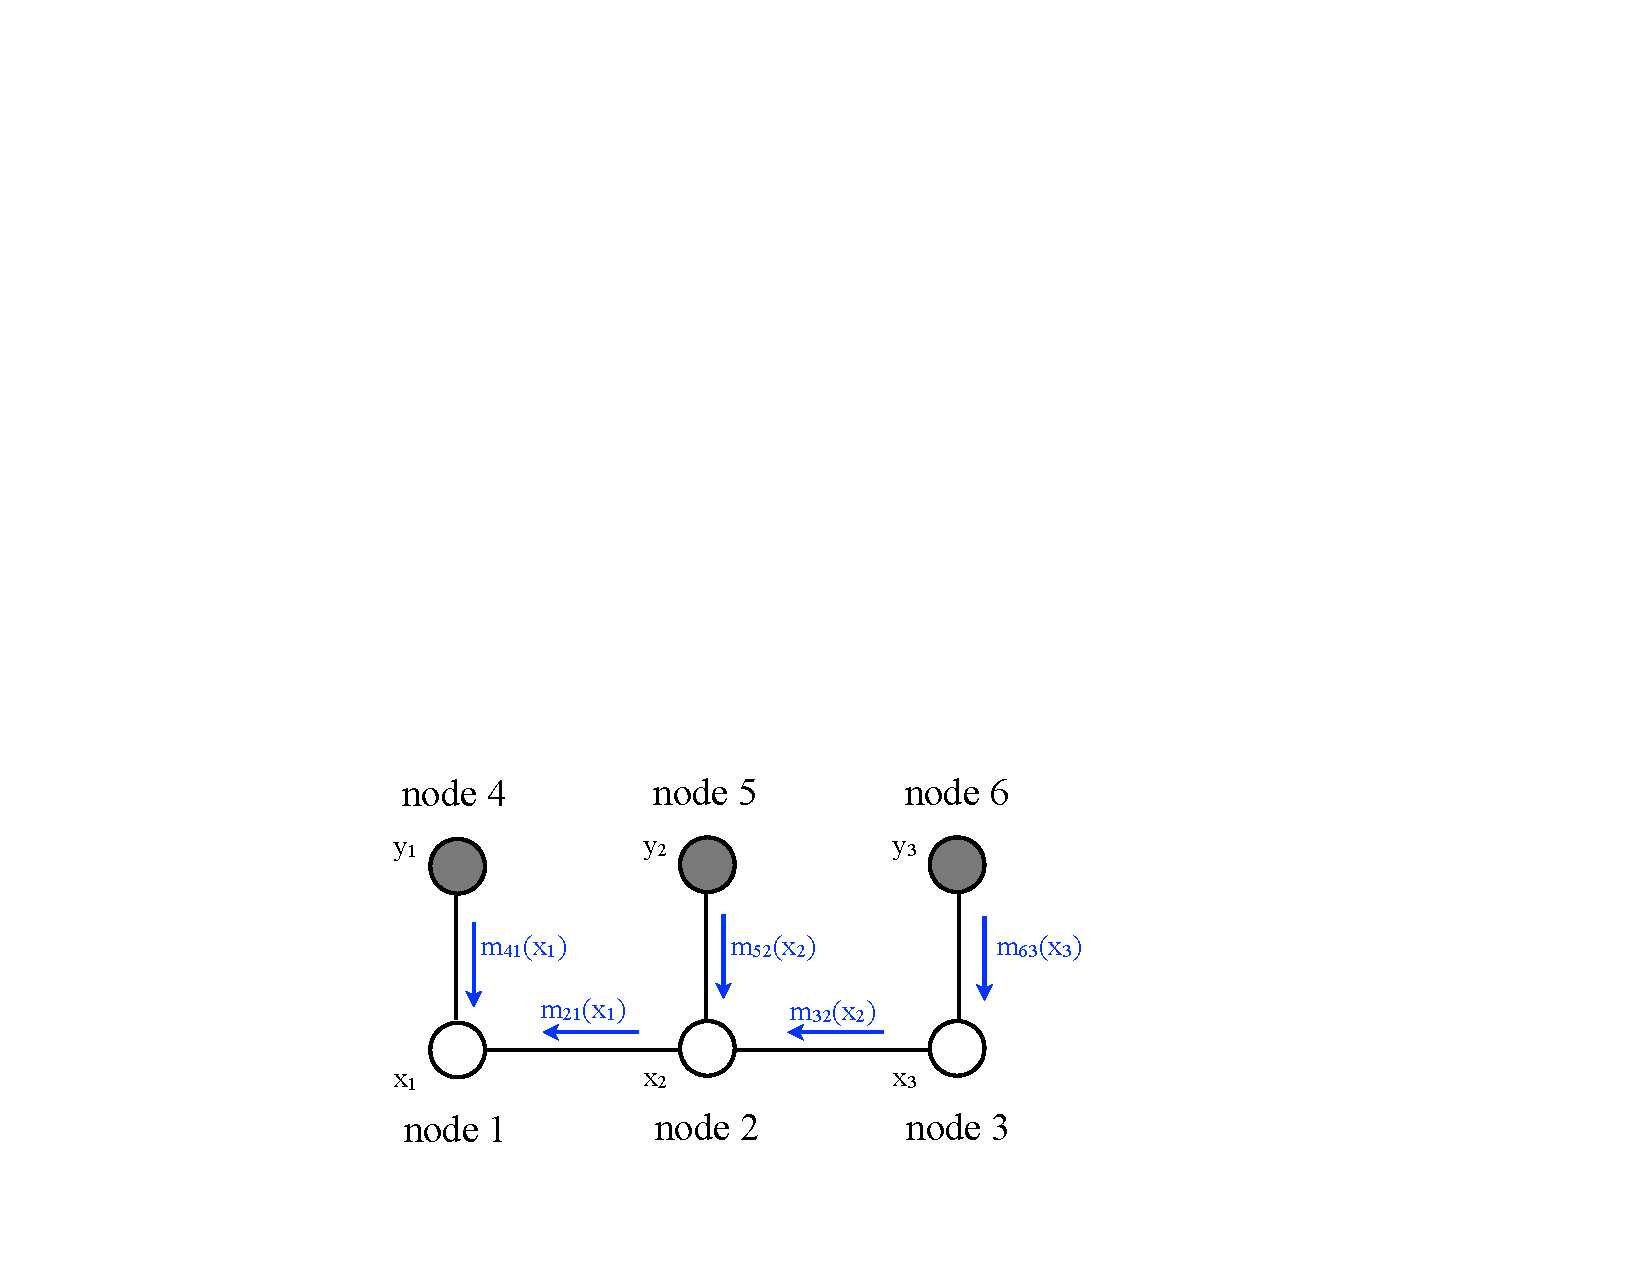
\includegraphics[width=0.5\linewidth]{figures/graphical_models/3bpc2.pdf}} 
\caption{Summary of the messages (partial sums) for a simple belief propagation example.} 
\label{fig:3bpc}
\end{figure}

\subsection{Derivation of Message-Passing Rule}
\label{sect:bpRules}

We'll describe belief propagation only for the special case of
graphical models with pairwise potentials.  
The clique potentials between neighboring nodes are $\psi_{ij}(x_j, x_i)$.
Extensions to higher-order
potentials is straightforward.  (Convert the
graphical model into one with only pairwise potentials.  This can be
done by augmenting the state of some nodes to encompass several others,
until the remaining nodes only need pairwise potential functions in
their factorization of the joint probability.)  You can find formal
derivations of belief propagation in \cite{Jordan98,Koller2009}.

Consider \fig{\ref{fig:bpmotivator2}}, showing a section of a general network with pairwise potentials.  There is a network of $N+1$
nodes, numbered $0$ through $N$ and we will marginalize over nodes
$x_1 \ldots x_N$.  \Fig{\ref{fig:bpmotivator2}}{a} shows the
marginalization equation for a network of variables with discrete states. (For continuous variables, integrals replace the summations). If we assume the nodes form a tree, we can
distribute the marginalization sum
past nodes for which the sum is a constant value to obtain the sums
depicted in \fig{\ref{fig:bpmotivator2}}{b}.  

We define a {\bf belief propagation message}:
A message $m_{ij}$, from node $i$ to node $j$, is the sum of the
 probability over all states of all
nodes in the subtree that leaves node $i$ and does not include node $j$.

Referring to \fig{\ref{fig:bpmotivator2}}{a}, shows the desired
marginalization sum over a network of pairwise cliques.   
We can pass the summations over node states through nodes that are
constant over those summations, arriving at the factorization shown in
\fig{\ref{fig:bpmotivator2}}{b}.  Remembering that the message from node $j$ to node $i$ is the sum
over the tree leaving node $j$, we can then read-off the recursive
belief propagation message update rule by marginalizing over the state probabilities at node $j$ in 
\fig{\ref{fig:bpmotivator2}}. As illustrated in \fig{\ref{fig:bpmotivator2}}, messages $m_{j+1,j}$ and $m_{kj}$ correspond to partial sums over nodes indicated in the graph: 
  $m_{j+1,j} = \sum_{x_{j+1} \ldots x_{k-1}}$ and 
  $m_{kj} = \sum_{x_k \ldots x_N}$.  Marginalization over the states of all nodes leaving node $j$, not including node $i$, leads to \eqn{\ref{eq:bpupdate}}, the belief propagation message passing rule.

\begin{figure}
\centerline{
\sublabel{a}{
%\centerline{
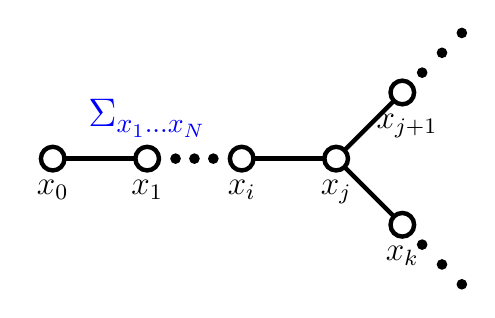
\begin{tikzpicture}[scale=0.6]
\draw [ultra thick] (-2,0) -- (0,0);
\draw [ultra thick, fill=white] (-2,0) circle [radius=0.25];
\node [below] at (-2,-0.25) {\large $x_{0}$};
\node [above, blue] at (0,0.25) {\Large $\Sigma_{x_1 \ldots x_N}$};
\draw [ultra thick, fill=white] (0,0) circle [radius=0.25];
\node [below] at (0, -0.25) {\large $x_1$};
\draw [fill] (0.6,0) circle [radius=0.1];
\draw [fill] (1,0) circle [radius=0.1];
\draw [fill] (1.4 ,0) circle [radius=0.1];
\draw [ultra thick] (2,0) -- (4,0);
\draw [ultra thick, fill=white] (2,0) circle [radius=0.25];
\node [below] at (2,-0.25) {\large $x_{i}$};
\draw [ultra thick] (4,0) -- (5.4,1.4);
\draw [ultra thick] (4,0) -- (5.4,-1.4);
\draw [ultra thick, fill=white] (4,0) circle [radius=0.25];
\node [below] at (4,-0.25) {\large $x_j$};
% \draw [fill] (4.6,0) circle [radius=0.1];
% \draw [fill] (5,0) circle [radius=0.1];
% \draw [fill] (5.4 ,0) circle [radius=0.1];
\draw [ultra thick,fill=white] (5.4,1.4) circle [radius=0.25];
\draw [fill] (5.82,1.82) circle [radius=0.1];
\draw [fill] (6.24,2.24) circle [radius=0.1];
\draw [fill] (6.66 ,2.66) circle [radius=0.1];
\node [below] at (5.5,1.15) {\large $x_{j+1}$};
\draw [ultra thick,fill=white] (5.4,-1.4) circle [radius=0.25];
\node [below] at (5.4,-1.65) {\large $x_k$};
\draw [fill] (5.82,-1.82) circle [radius=0.1];
\draw [fill] (6.24,-2.24) circle [radius=0.1];
\draw [fill] (6.66 ,-2.66) circle [radius=0.1];
\end{tikzpicture}}
%}
\sublabel{b}{
%\centerline{
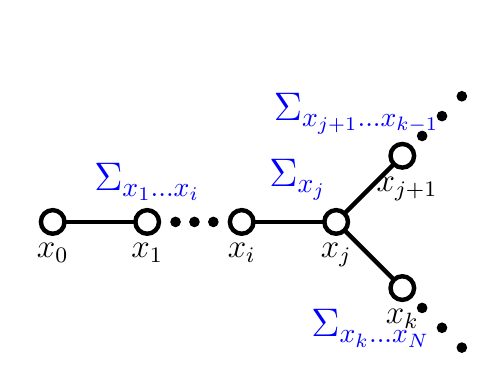
\begin{tikzpicture}[scale=0.6]
\draw [ultra thick] (-2,0) -- (0,0);
\draw [ultra thick, fill=white] (-2,0) circle [radius=0.25];
\node [below] at (-2,-0.25) {\large $x_{0}$};
\node [above, blue] at (0,0.25) {\Large $ \Sigma_{x_1 \ldots x_{i}}$};
\draw [ultra thick, fill=white] (0,0) circle [radius=0.25];
\node [below] at (0, -0.25) {\large $x_1$};
\draw [fill] (0.6,0) circle [radius=0.1];
\draw [fill] (1,0) circle [radius=0.1];
\draw [fill] (1.4 ,0) circle [radius=0.1];
\draw [ultra thick] (2,0) -- (4,0);
\draw [ultra thick, fill=white] (2,0) circle [radius=0.25];
\node [below] at (2,-0.25) {\large $x_{i}$};
\draw [ultra thick] (4,0) -- (5.4,1.4);
\draw [ultra thick] (4,0) -- (5.4,-1.4);
\draw [ultra thick, fill=white] (4,0) circle [radius=0.25];
\node [below] at (4,-0.25) {\large $x_j$};
\node [above left, blue] at (4, 0.25) {\Large $ \Sigma_{x_{j}}$};
\draw [ultra thick,fill=white] (5.4,1.4) circle [radius=0.25];
\draw [fill] (5.82,1.82) circle [radius=0.1];
\draw [fill] (6.24,2.24) circle [radius=0.1];
\draw [fill] (6.66 ,2.66) circle [radius=0.1];
% to add space between the figures
\draw [fill, white] (6.66,4) circle [radius=0.1];
\node [below] at (5.5,1.15) {\large $x_{j+1}$};
\node [above left, blue] at (6.4, 1.65) {\Large $ \Sigma_{x_{j+1} \ldots x_{k-1}}$};
\draw [ultra thick,fill=white] (5.4,-1.4) circle [radius=0.25];
\node [below] at (5.4,-1.65) {\large $x_k$};
\node [below left, blue] at (6.2, -1.65) {\Large $ \Sigma_{x_{k} \ldots x_{N}}$};
\draw [fill] (5.82,-1.82) circle [radius=0.1];
\draw [fill] (6.24,-2.24) circle [radius=0.1];
\draw [fill] (6.66 ,-2.66) circle [radius=0.1];
\end{tikzpicture}}
%}
}
\caption{Example motivating belief propagation update rule. (a)
  Marginalization of a graph with no loops.  (b) Shows how the partial sums at $x_j$ distribute over nodes.} 
\label{fig:bpmotivator2}
\end{figure}


To compute the message from node $j$ to node $i$:
\begin{enumerate}
\item Multiply together all messages (independent probabilities) coming in to node $j$, except for
 the message from node $i$ back to node $j$,
\item Multiply by the pairwise compatibility function $\psi_{ij}(x_i, x_j)$ (also independent of the other multiplicands).
\item Marginalize over the variable $x_j$.
\end{enumerate}
These steps are summarized in this equation to compute the message from node $j$ to node $i$:
\begin{equation} 
m_{ji}(x_i) = \sum_{x_j} \psi_{ij} (x_i, x_j) 
\prod_{k\in \eta(j) \mbox{\textbackslash}   i} m_{kj}(x_j)
\label{eq:bpupdate}
\end{equation} 
where $\eta(j) \mbox{\textbackslash}   i$ means ``the neighbors of
node $j$ except for node $i$.''  \Fig{\ref{fig:bpdiscrete}} shows this
equation in a graphical form.  Any local potential functions
$\phi_{j}(x_j)$ are treated as an additional message into node $j$, that is, $m_{0j}(x_j) = \phi_{j}(x_j)$.
For the case of continuous variables, the
sum over the states of $x_j$ in \eqn{\ref{eq:bpupdate}} is replaced by an integral over the
domain of $x_j$.

\begin{figure}
\centerline{
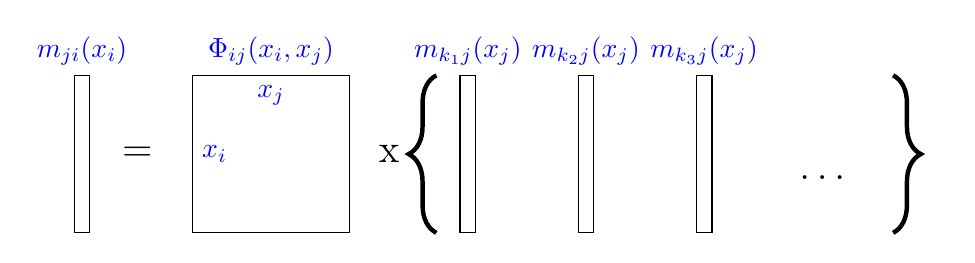
\begin{tikzpicture}
\draw [draw=black]  (-2.8, 2) rectangle (-3, 0);
\node [above, blue] at (-2.9, 2) {$m_{ji}(x_i)$};
\node at (-2.2,1) {\Large  $ =$};
\draw [draw=black]  (-1.5, 2) rectangle (0.5, 0);
\node [above,blue] at (-0.5, 2) {$\Phi_{ij}(x_i, x_j)$};
\node [below, blue] at (-0.5, 2) {$x_j$};
\node [right, blue] at (-1.5, 1) {$x_i$};
\node at (1.0,1) {\Large  $\mbox{x}$};
\draw [draw=black]  (1.9, 2) rectangle (2.1, 0);
\node [above, blue] at (2.0, 2) {$m_{{k_1}j}(x_j)$};
\node at (2.6,1) {\Large  $\hadamard$};
\draw [draw=black]  (3.4, 2) rectangle (3.6, 0);
\node [above, blue] at (3.5, 2) {$m_{{k_2}j}(x_j)$};
\node at (4.1,1) {\Large  $\hadamard$};
\draw [draw=black]  (4.9, 2) rectangle (5.1, 0);
\node [above, blue] at (5.0, 2) {$m_{{k_3}j}(x_j)$};
\node at (5.6,1) {\Large  $\hadamard$};
\node at (6.5,0.7) {\Large  $\ldots$};

% Adding large parentheses
\draw[decoration={brace, amplitude=10pt, mirror}, decorate, ultra thick] (1.6,2) -- node[right=12pt] {} (1.6,0);
\draw[decoration={brace, amplitude=10pt}, decorate, ultra thick] (7.4,2) -- node[right=12pt] {} (7.4,0);
\end{tikzpicture}}
\caption{Pictorial depiction of belief propagation message passing
 rules of \eqn{\ref{eq:bpupdate}}, where $\hadamard$ indicates elementwise multiplication (i.e., the Hadamard product).  
 % To send a message from node j to
%  node i:  We term-by-term multiply (shown by .*) the messages (column vectors)
%  coming in to node j, then matrix multiply (shown by $\mbox{x}$)
% the resulting column vector by the compatibility matrix $\Phi_{ij}(x_i, x_j)$ to obtain $m_{ji}(x_i)$.
} 
\label{fig:bpdiscrete}
\end{figure}


As mentioned previously, BP messages are partial sums in the
marginalization calculation.  The arguments of messages are always the
state of the node that the message is going to.
(BP follows the ``nosey neighbor rule'' (from Brendan Frey, Univ. Toronto): Every node is a house in some neighborhood. Your nosey neighbor says to you, ``Given what I've seen myself and everything I’ve heard from my neighbors, here’s what I think is going on inside
your house.'' (That metaphor especially makes sense if one has teenaged children.)


\subsection{Marginal Probability}

\begin{figure}
\centerline{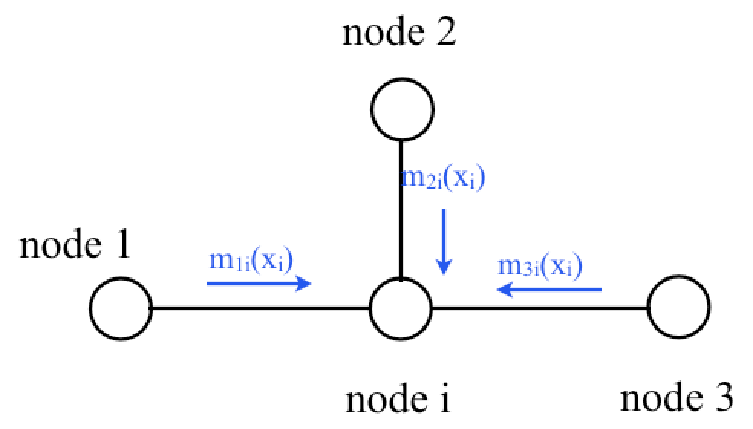
\includegraphics[width=0.48\linewidth]{figures/graphical_models/bpi.pdf}} 
\caption{To compute the marginal probability at node $i$, we multiply
 together all the incoming messages at that node:  
$p_{i}(x_i) =  \prod_{j\in \eta(i)}  m_{ji}(x_i)$, including any local potential terms $\phi_i(x_i)$ as another message.
}
\label{fig:bpi}
\end{figure}
 
The marginal probability at a node $i$, \eqn{\ref{eq:discreteMarginalization}}, is the sum over the joint probabilities of all states except those of $x_i$.  Because we assume the network has no loops, the conditional
independence structure assures us that marginal probability at a node $i$ is the product of the sum of all states of all nodes in each
subtree connected to node $i$: Conditioned on node $i$, the probabilities within each subtree are independent. Thus the marginal probability at node $i$
is the product of all the incoming messages:
\begin{equation}
p_{i}(x_i) = \prod_{j\in \eta(i)}  m_{ji}(x_i)
\label{eq:bpmarginal}
\end{equation}
(We include the local clique potential at node $i$, $\psi_i(x_i)$, as
one of the messages in the product of all messages into node $i$).


\subsection{Message Update Sequence}
To find all the messages, how do we invoke the recursive BP update rule, \eqn{\ref{eq:bpupdate}}?  We can apply \eqn{\ref{eq:bpupdate}}
whenever all the incoming messages in the BP update rule are defined.  If there
 are no incoming messages to a node, then its outgoing message is
well-defined in the update rule.  This lets us start the recursive algorithm.

A node can send a message whenever all the incoming messages it needs
have been computed.  We can compute the outgoing messages
from leaf nodes in the graphical model tree, since they have no
incoming messages other than from the node to which they are sending a
message, which doesn't enter in the outgoing message computation.  Two
natural message passing protocols are consistent with that rule:
depth-first update, and parallel update.  In depth-first update, one
node is arbitrarily picked as the root.  Messages are then passed from
the leaves of the tree (leaves, relative to that root node) up to the
root, then back down to the leaves.  In parallel update, at each turn,
every node sends every outgoing message for which it has received all
the necessary incoming messages.  \Fig{\ref{fig:men}} depicts the
flow of messages for the parallel, synchronous update scheme and \Fig{\ref{fig:men2}} shows the flow for the same network, but with a depth-first update schedule.

Note that when computing marginals at many nodes, we reuse messages
with the BP algorithm.  A single message-passing sweep through all the
nodes lets us calculate the marginal at any node (using the
depth-first update rules to calculate the marginal at the root node).
A second sweep from the root node back to all the leaf nodes
calculates all the messages needed to find the marginal probability at
every node.  It takes only twice the number of computations to
calculate the incoming messages to every node, and thus the marginal probabilities everywhere, as it does to
calculate the incoming messages for the marginal probability at a single node.

\begin{figure}
\centerline{
\sublabel{a}{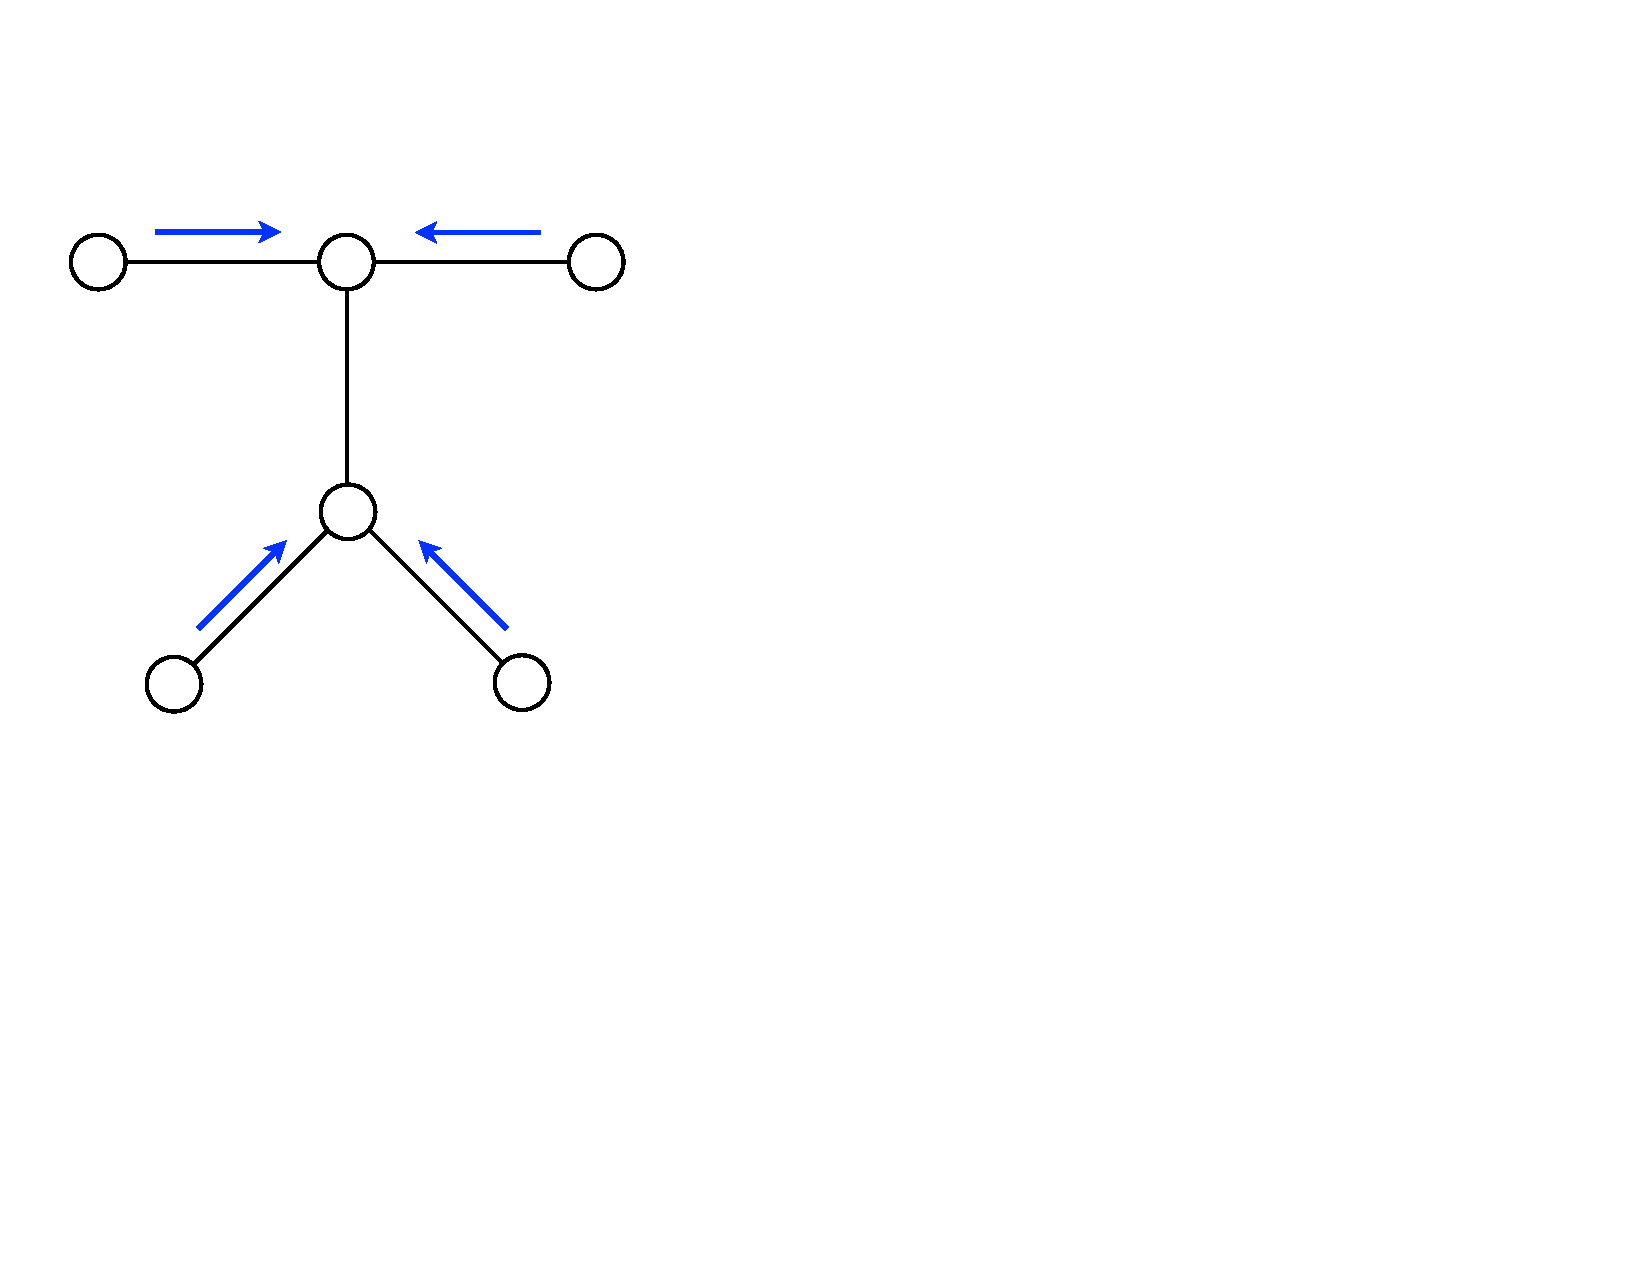
\includegraphics[width=0.20\linewidth]{figures/graphical_models/man1.pdf}}
\sublabel{b}{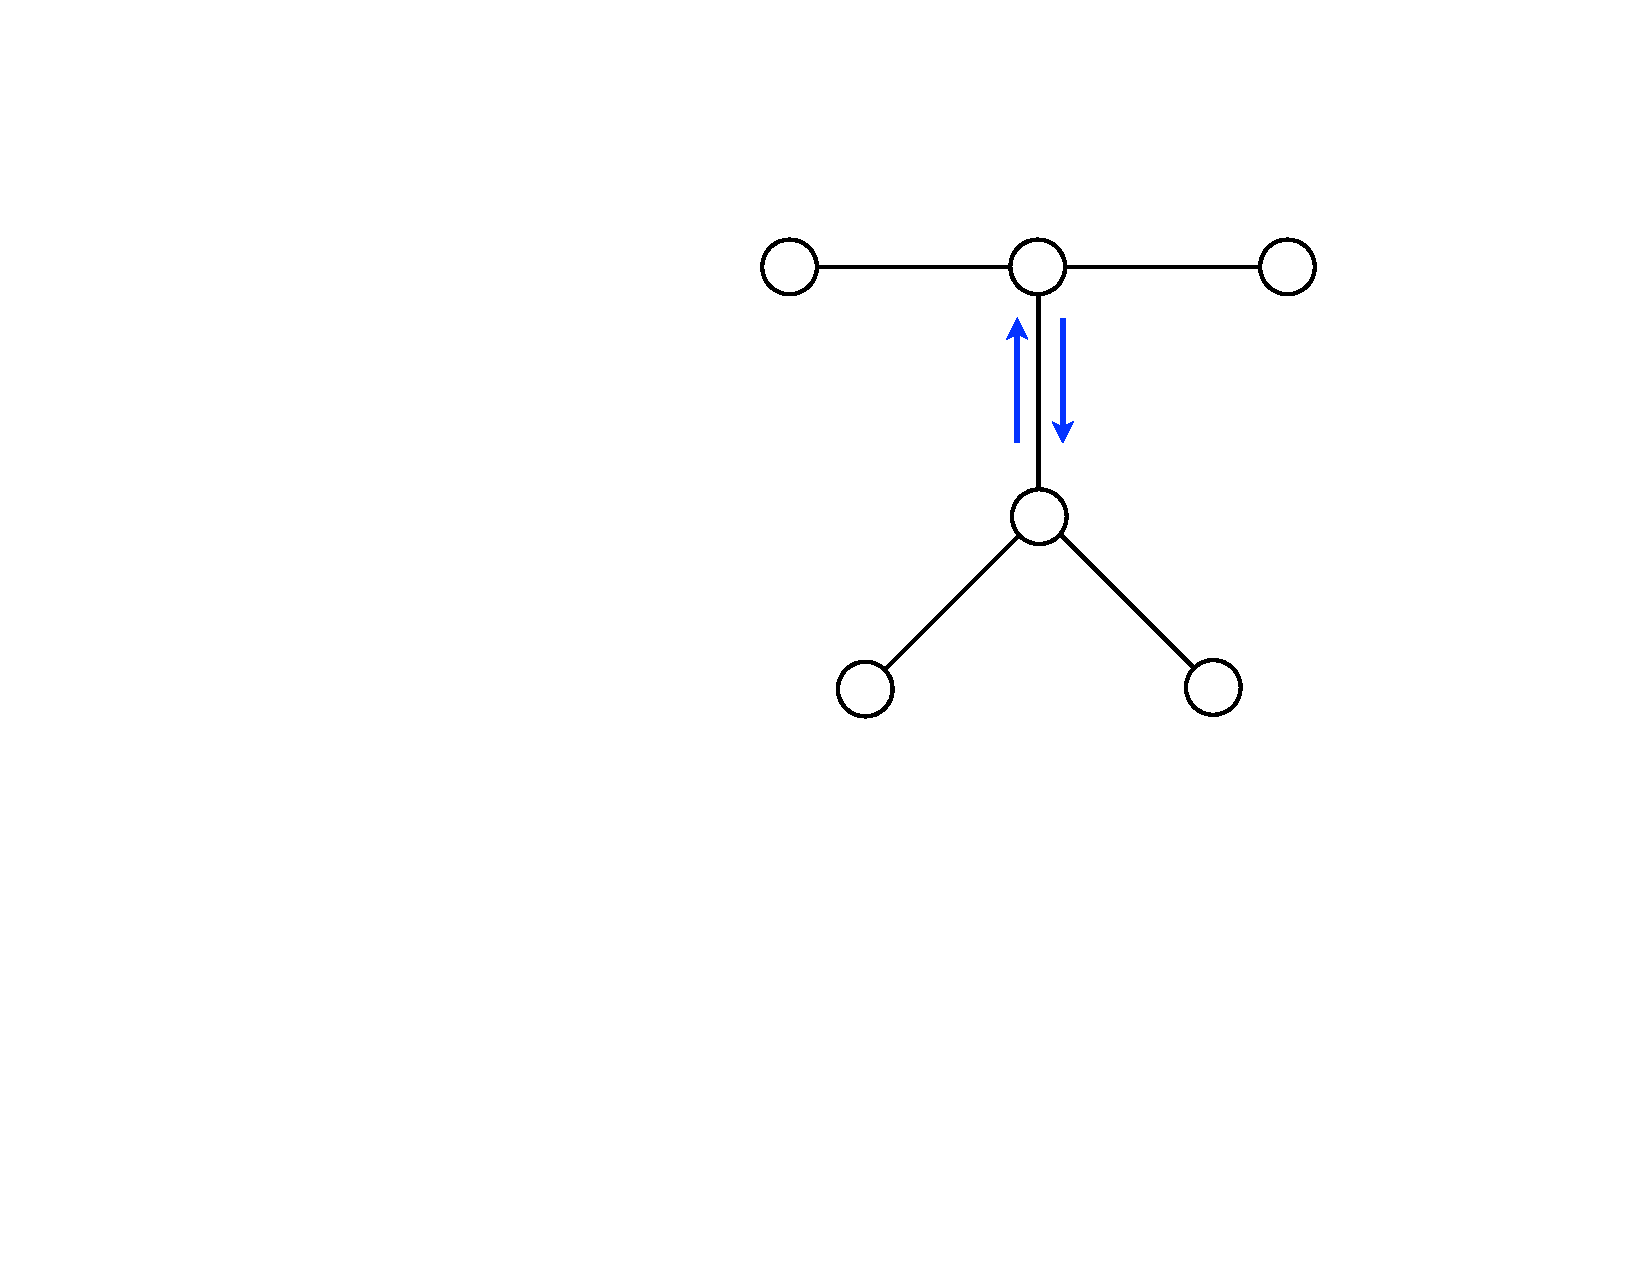
\includegraphics[width=0.20\linewidth]{figures/graphical_models/man2.pdf}}
\sublabel{c}{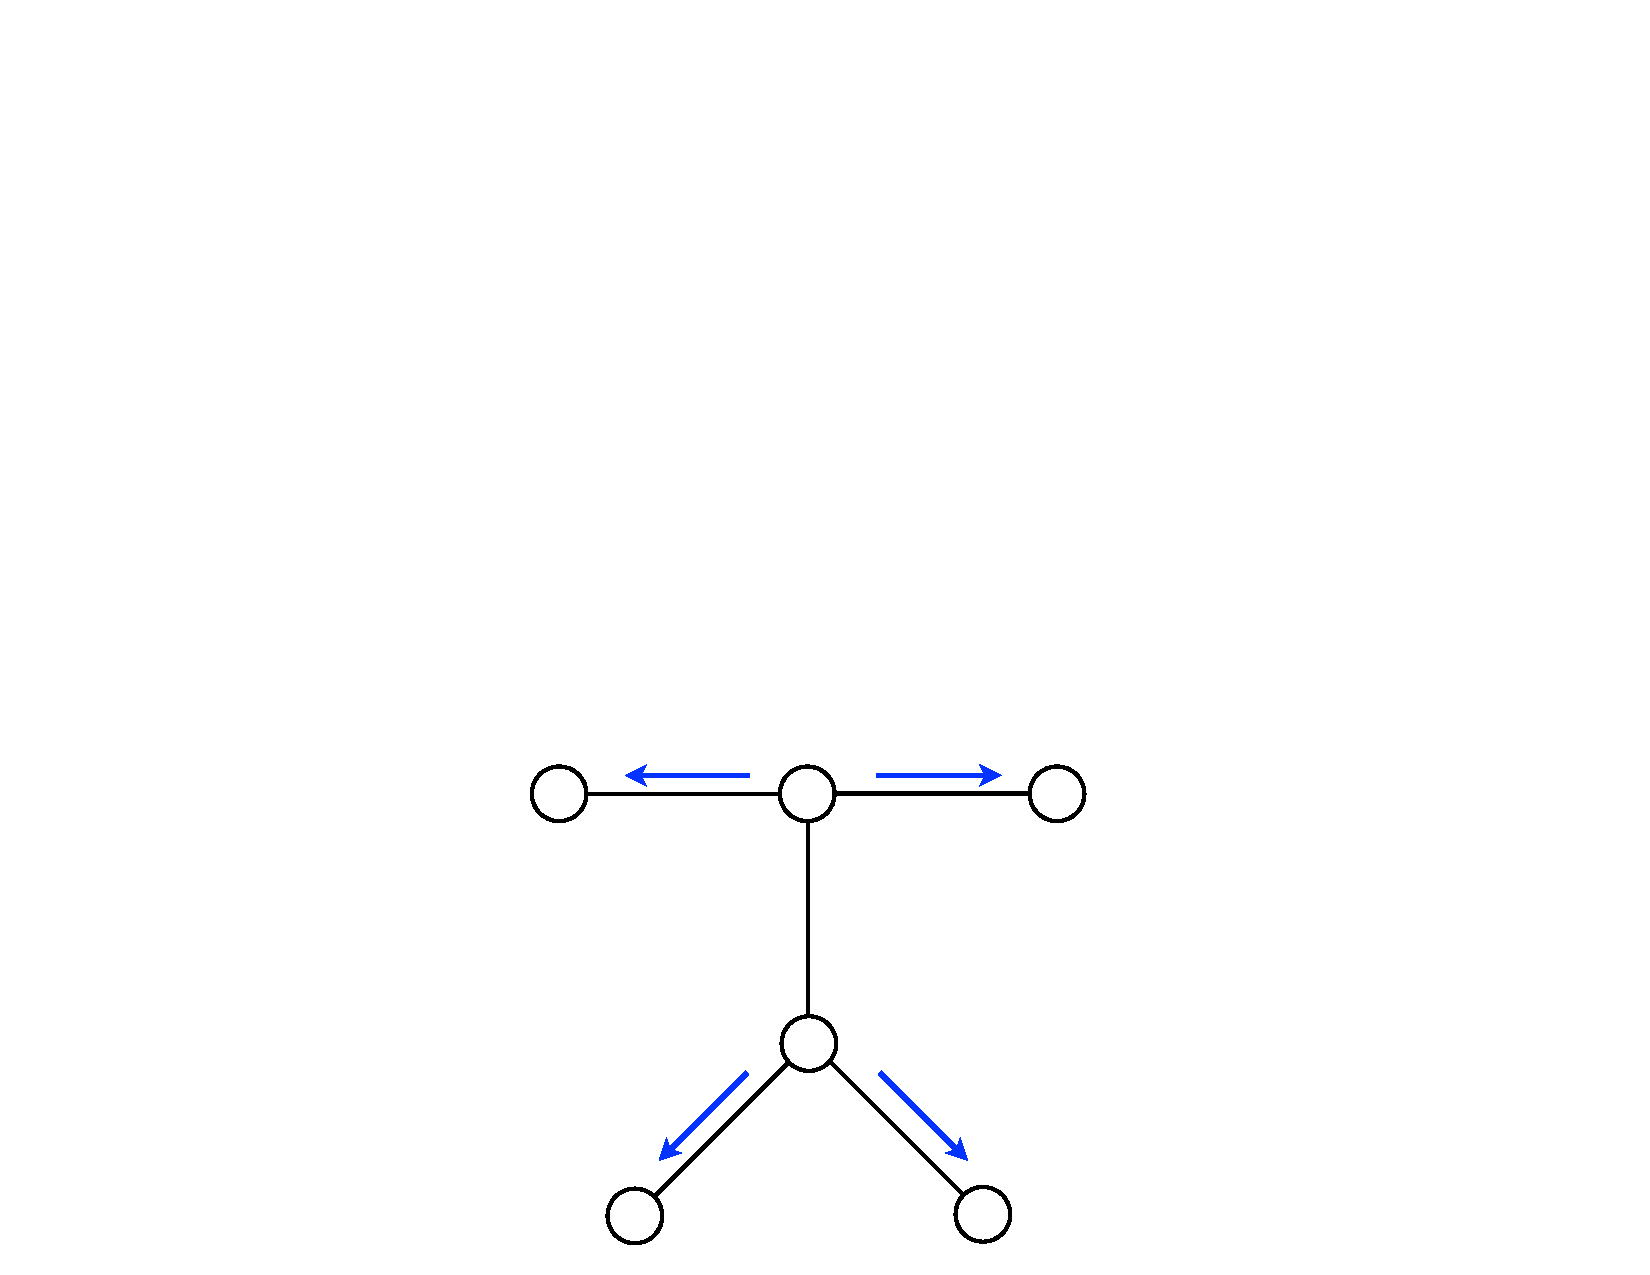
\includegraphics[width=0.20\linewidth]{figures/graphical_models/man3.pdf}}
}
\caption{{\bf Synchronous parallel update schedule} for BP message passing: Each node sends an outgoing message as soon as it receives the necessary incoming messages. Iterations: (a) one, (b) two, and (c) three.} 
\label{fig:men}
\end{figure}




\begin{figure}
\centerline{
\sublabel{a}{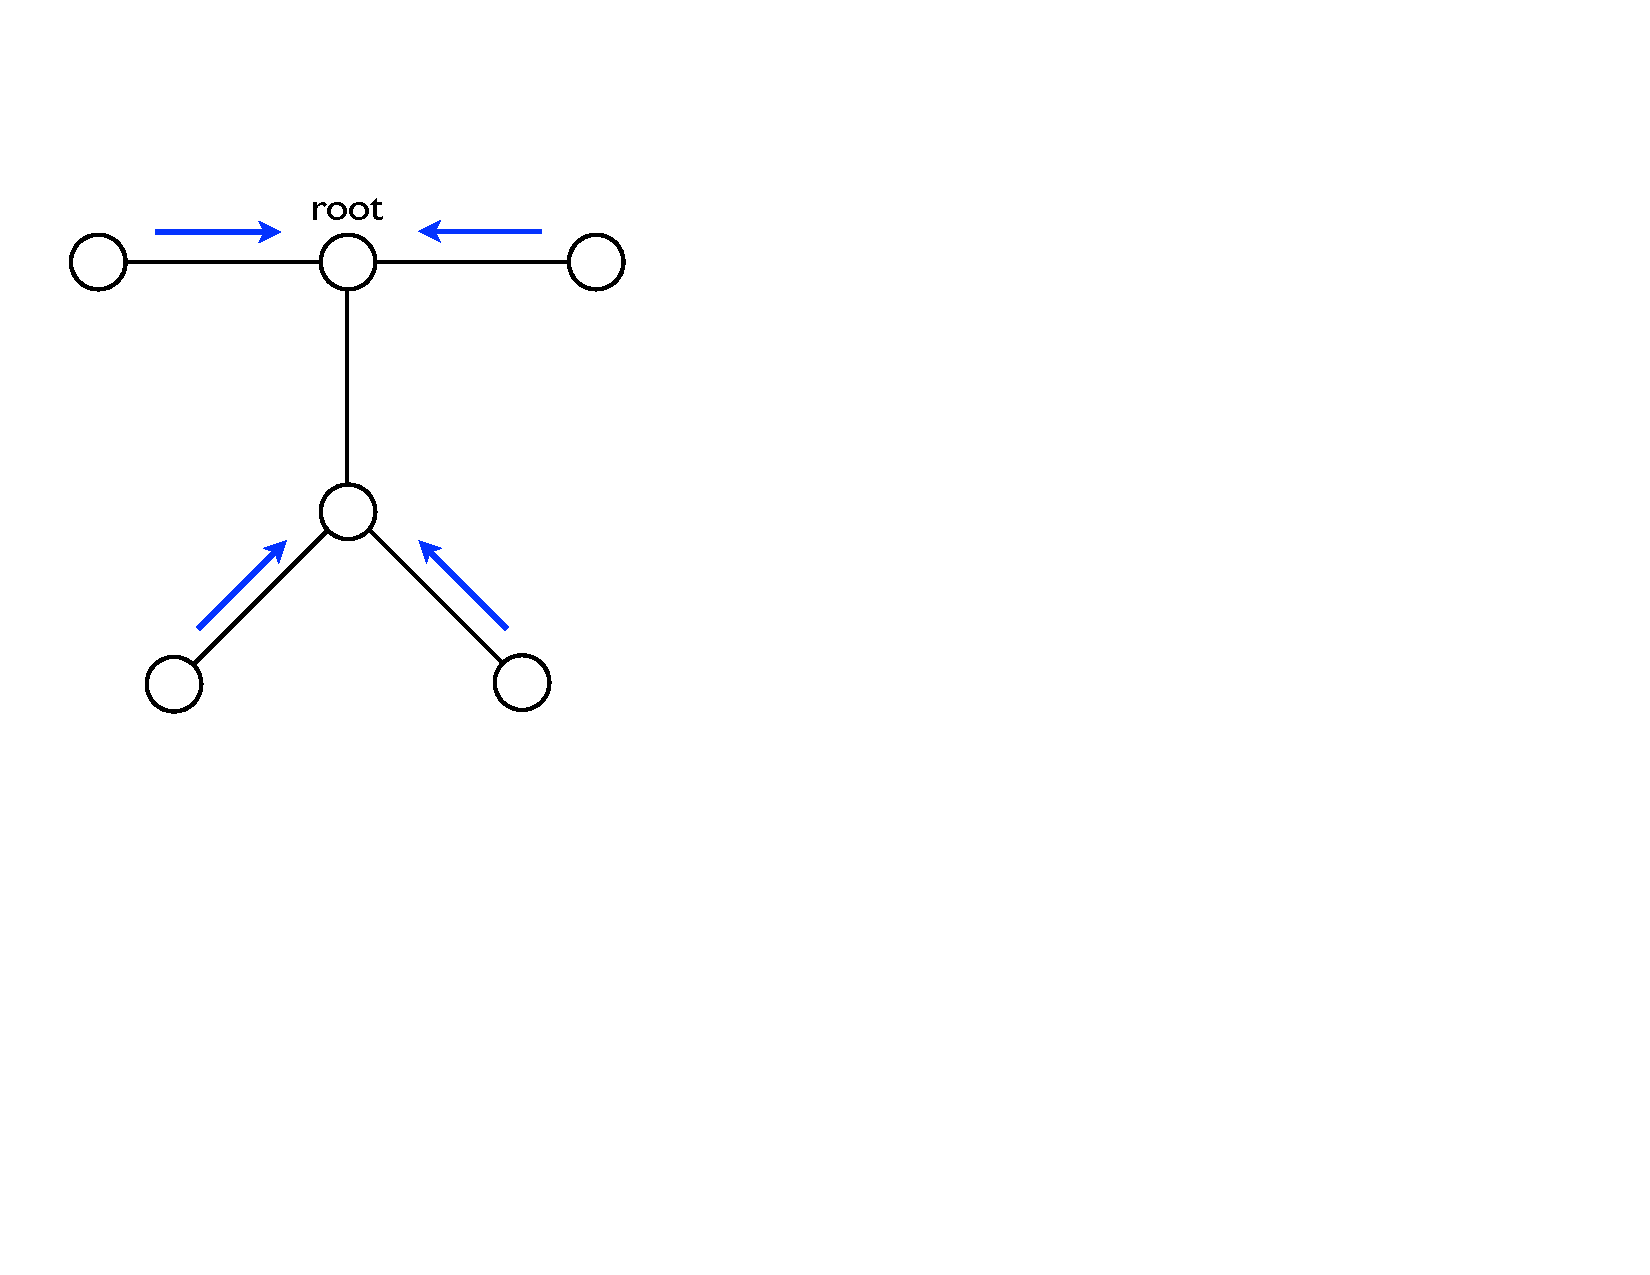
\includegraphics[width=0.20\linewidth]{figures/graphical_models/rootman1.pdf}}
\sublabel{b}{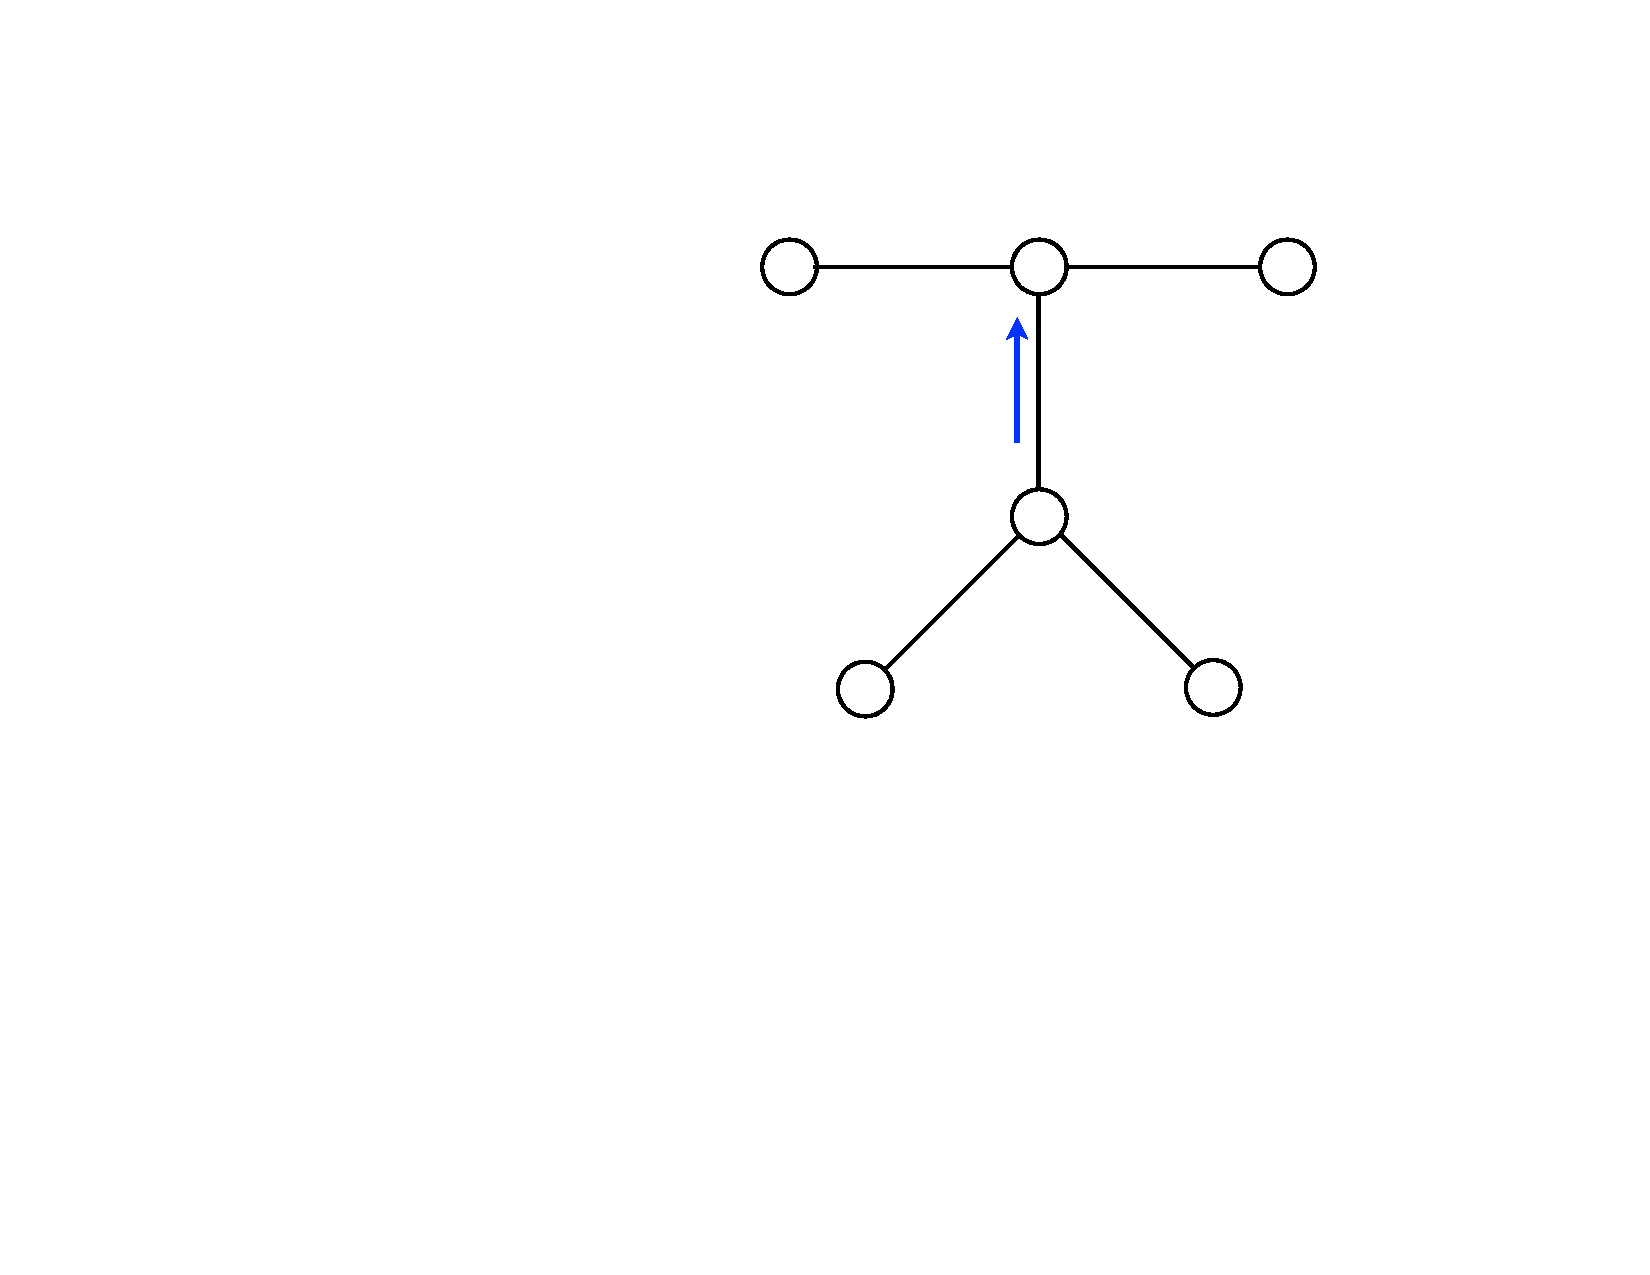
\includegraphics[width=0.20\linewidth]{figures/graphical_models/rootman2.pdf}}
\sublabel{c}{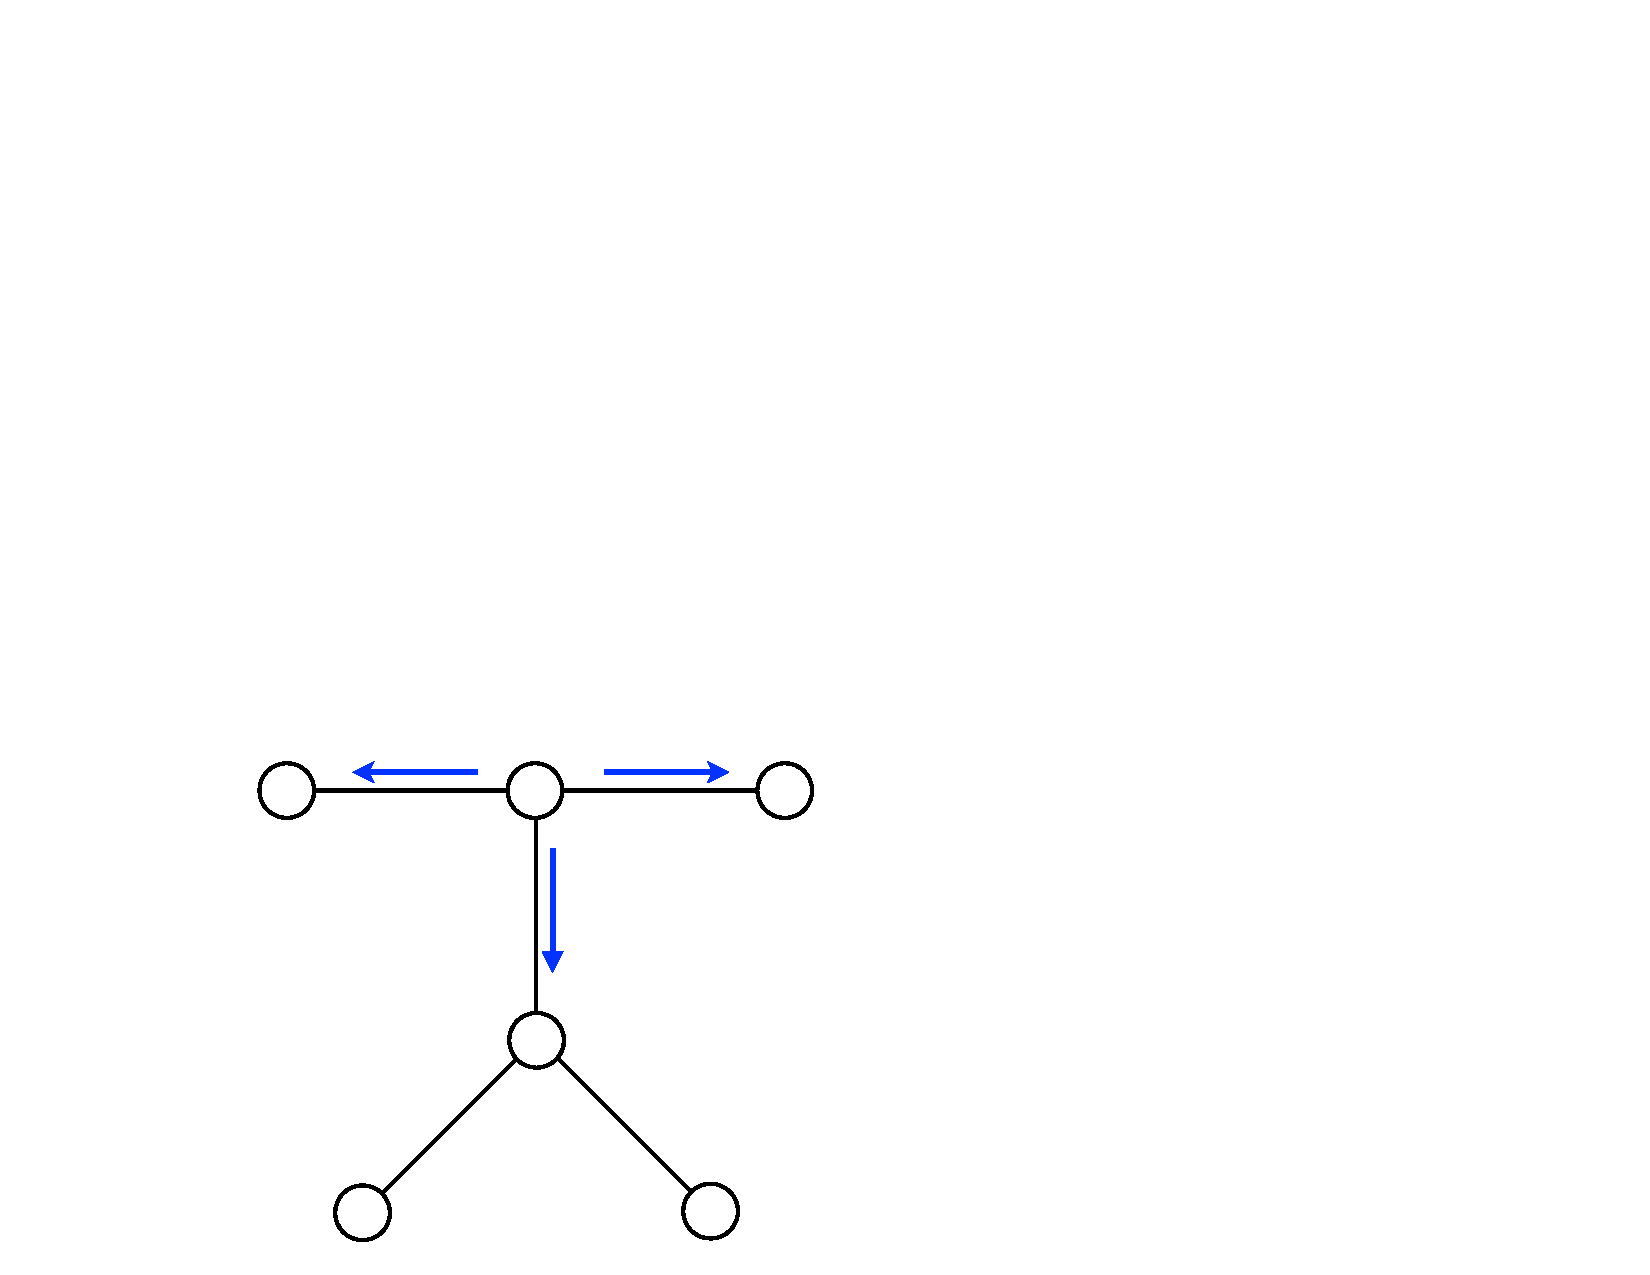
\includegraphics[width=0.20\linewidth]{figures/graphical_models/rootman3.pdf}}
\sublabel{d}{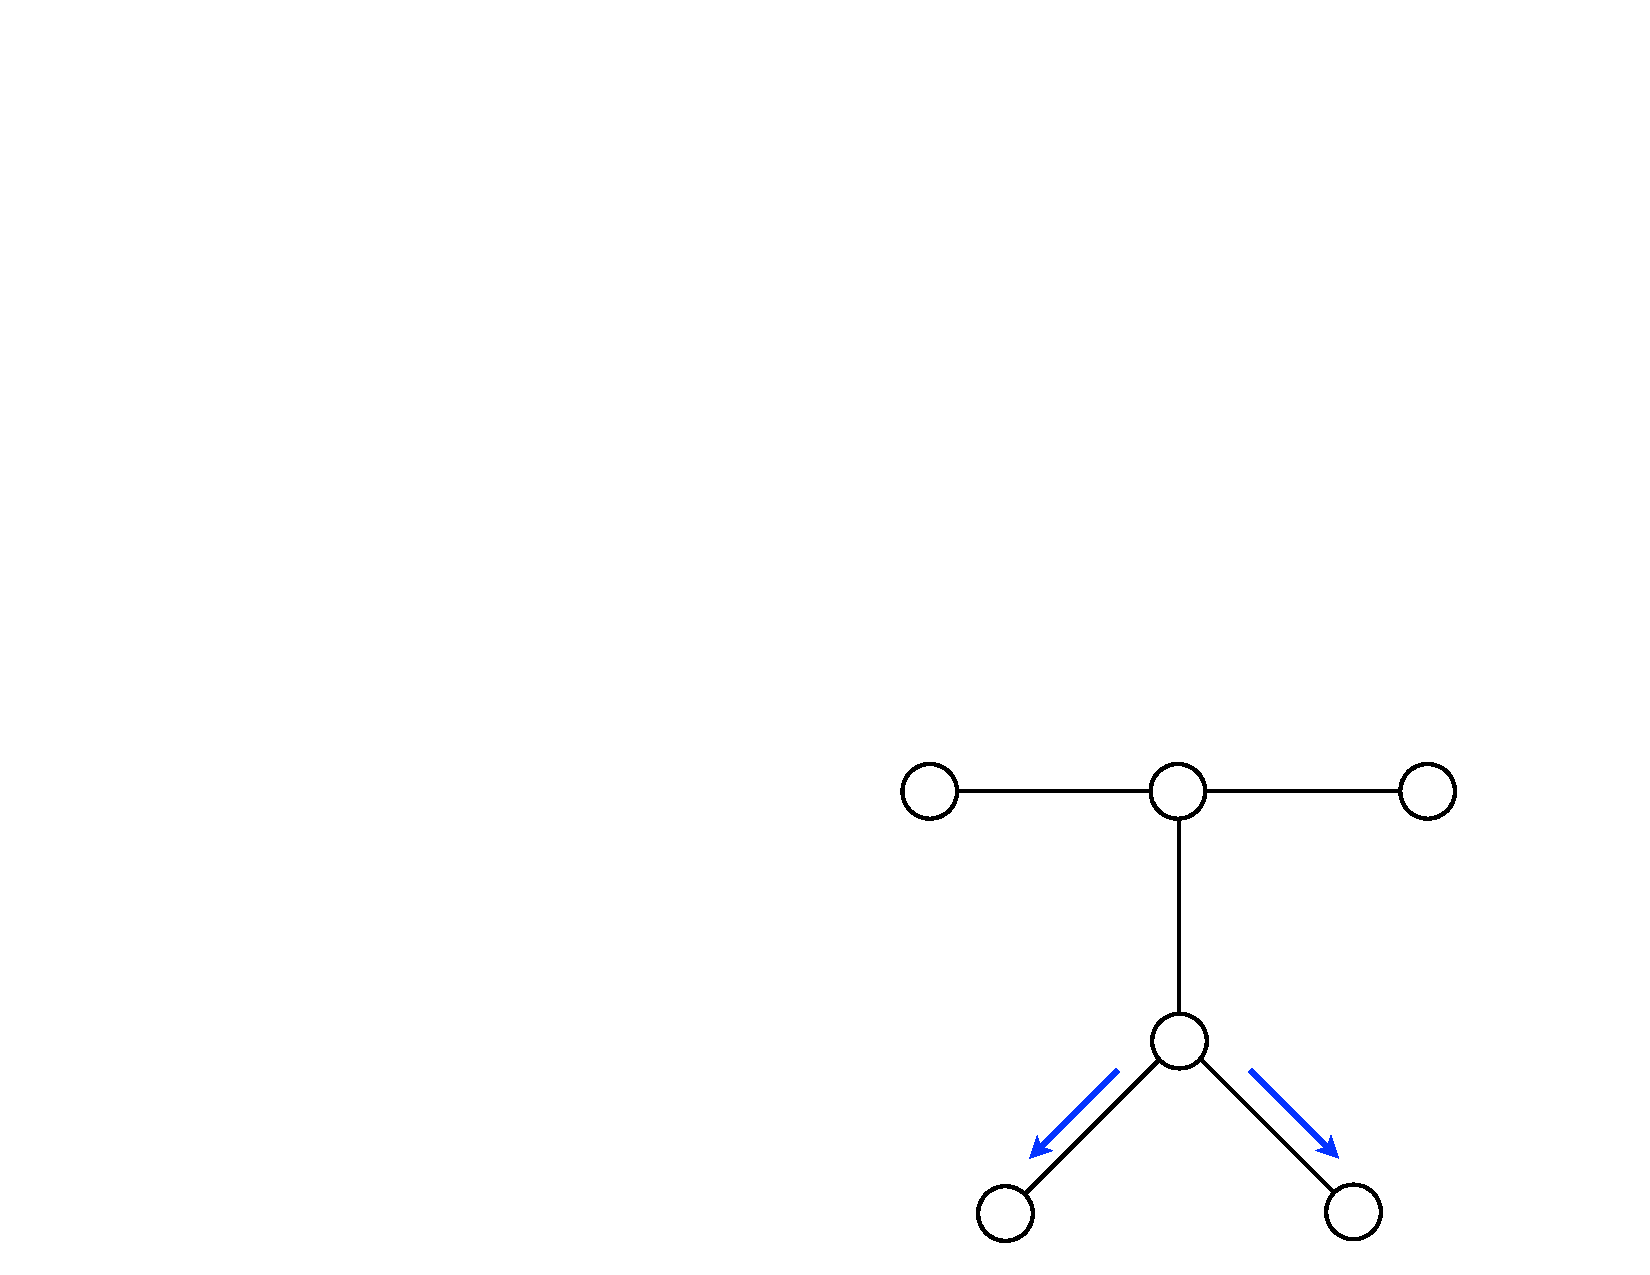
\includegraphics[width=0.20\linewidth]{figures/graphical_models/rootman4.pdf}}
}
\caption{
{\bf Depth-first BP message passing schedule}. Select a root node. (a) Start at leaves; (b) proceed to root; (c), perform an outgoing sweep; and (d) compute remaining messages, ending at leaf nodes.}
\label{fig:men2}
\end{figure}

\subsection{Example Belief Propagation Application: Stereo}

Assume that we want to compute the depth from a stereo image pair, such as the pair shown in figures~\ref{fig:canoe1}(a and b) and with their insets marked with the red rectangles, shown in figures~\ref{fig:canoe1}(c and d).   Assume that the two images have been rectified, as described in \chap{\ref{chap:stereo_vision}}, and consider the common scanline, marked in figures~\ref{fig:canoe1}(c and d) with a black horizontal line.  The luminance intensities of each scanline are plotted in figures~\ref{fig:canoe1}(e and f).  Most computer vision stereo algorithms \cite{Scharstein2002} examine multiple scanlines to compute the depth at every pixel, but to illustrate a simple example of belief propagation in vision, we will consider the stereo vision problem while considering only one scanline pair at a time.


\begin{figure}[t]
\centerline{
\sublabel{a}{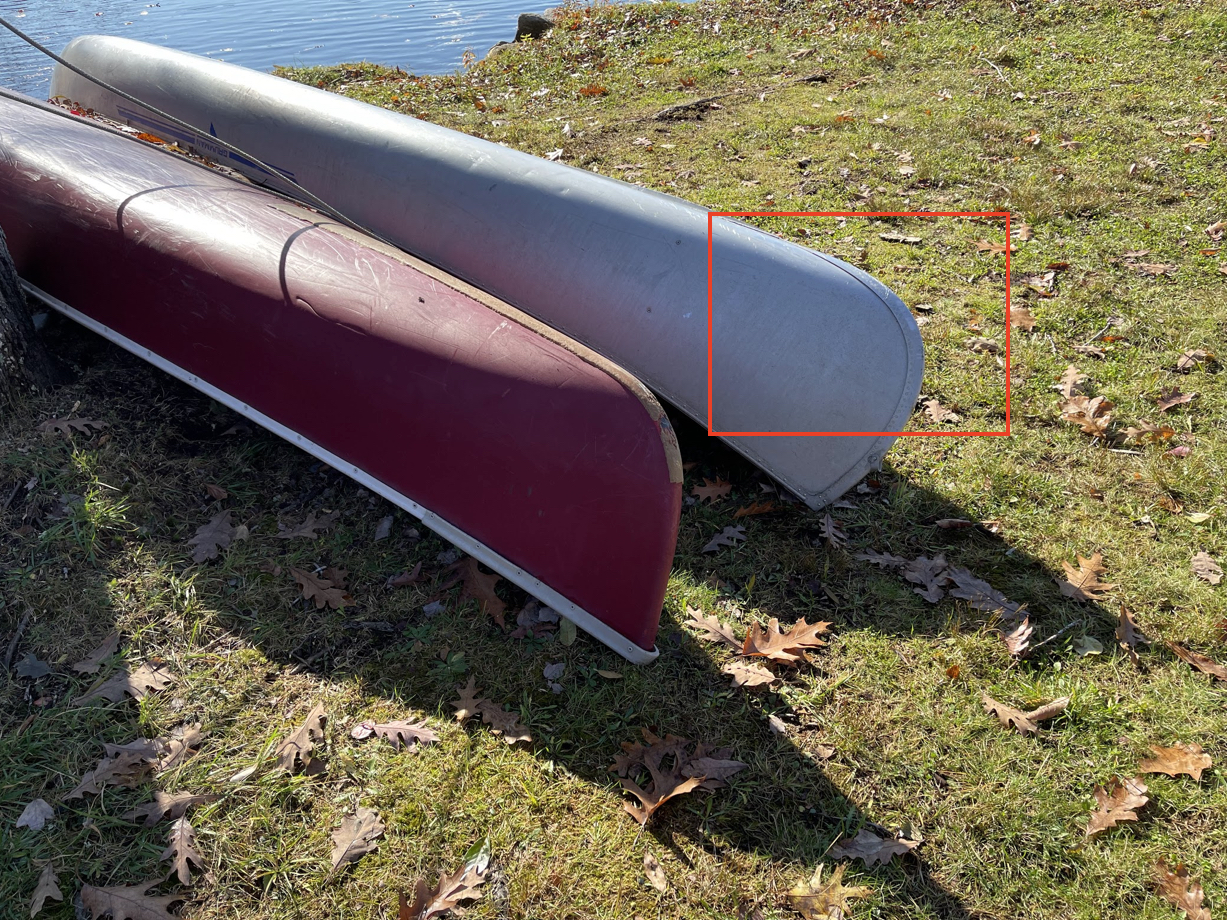
\includegraphics[width=0.40\linewidth]{figures/graphical_models/lcanoebig.jpg}}
\sublabel{b}{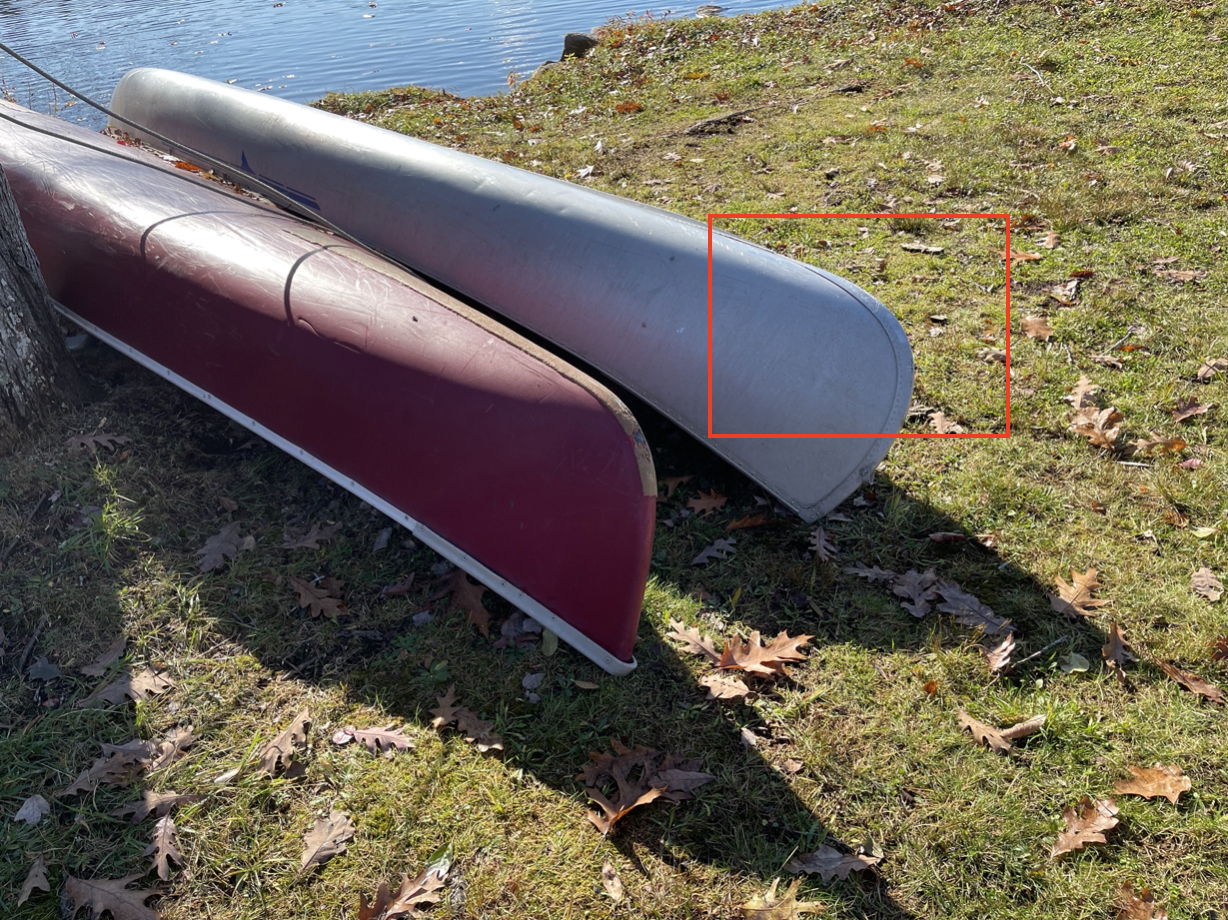
\includegraphics[width=0.40\linewidth]{figures/graphical_models/rcanoebig.jpg}}
}
\centerline{
\sublabel{c}{
\includegraphics[width=0.40\linewidth]{figures/graphical_models/lcanoe2.jpg}}
\sublabel{d}{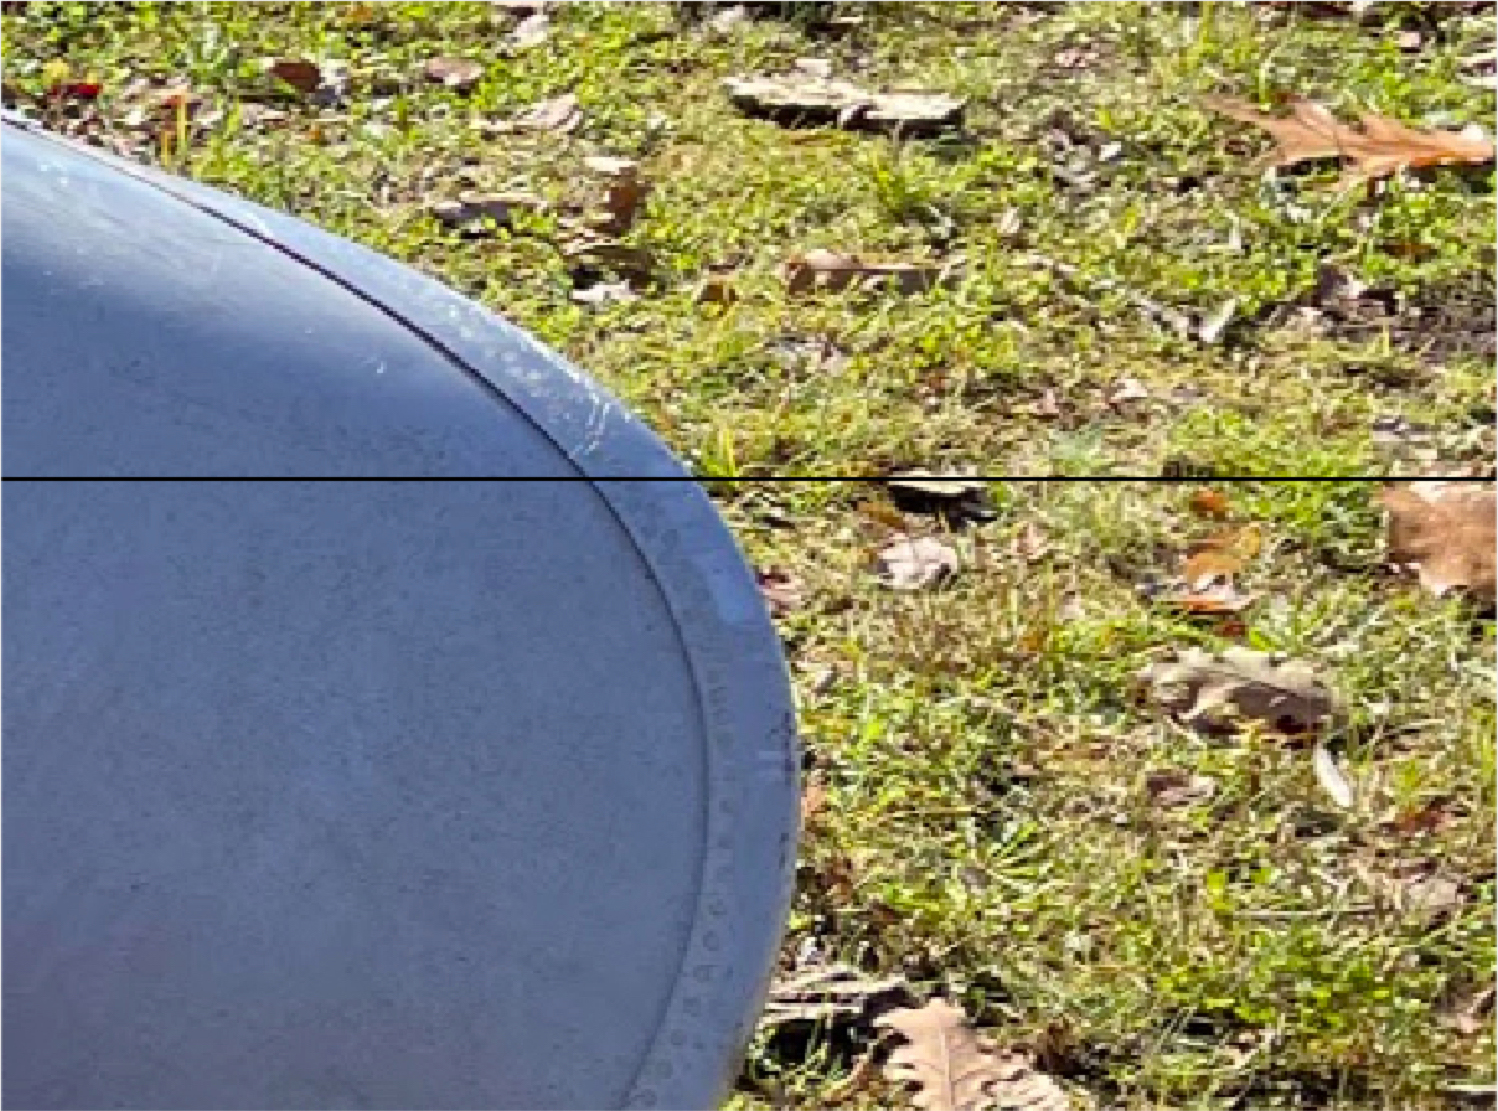
\includegraphics[width=0.40\linewidth]{figures/graphical_models/rcanoe2.jpg}}}
% \centerline{
% \sublabel{e} {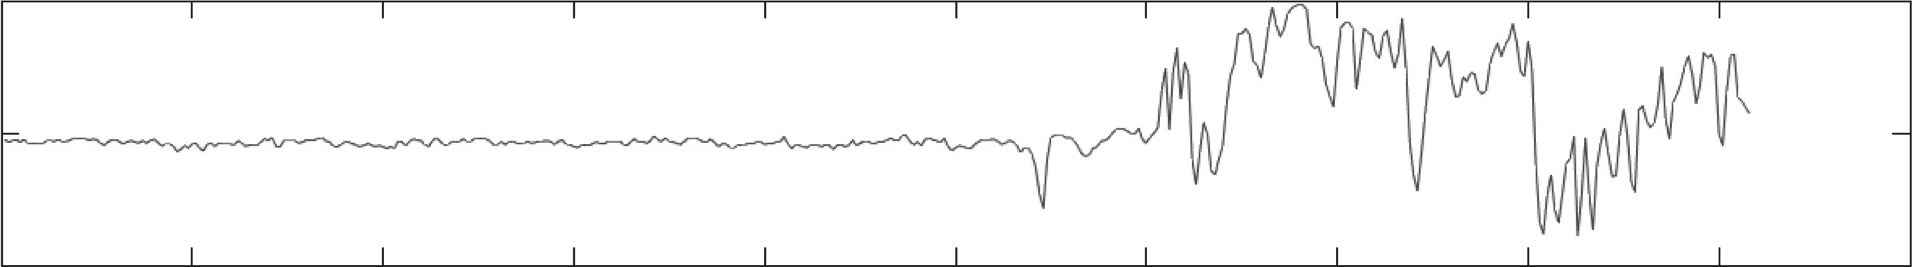
\includegraphics[width=0.30\linewidth]{figures/graphical_models/leftline.jpg}}
% \sublabel{f}{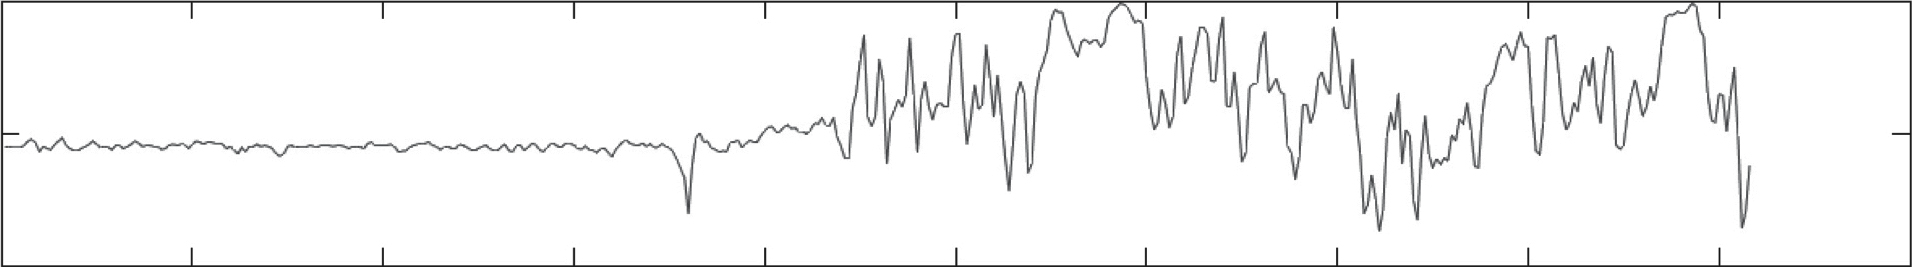
\includegraphics[width=0.30\linewidth]{figures/graphical_models/rightline.jpg}}}
\caption{(a) Left and (b) right camera images. (c and d): insets showing areas of analysis.}
\label{fig:canoe1}
\end{figure}

The graphical model that describes this stereo depth reconstruction for a single scanline is shown in \fig{\ref{fig:canoe3}}.  



\begin{figure}
\centerline{
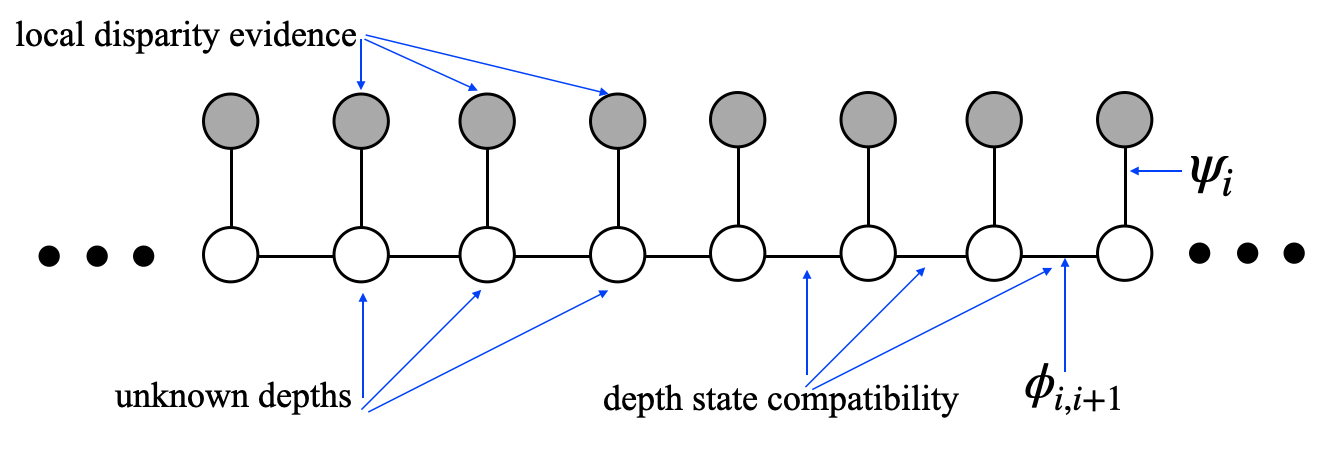
\includegraphics[width=0.80\linewidth]{figures/graphical_models/stereomodel2.jpg}
}
\caption{Graphical model for the posterior probability for stereo disparity offset between the left and right camera views from a stereo rig.}
\label{fig:canoe3}
\end{figure}

Each unfilled circle in the graphical model (\fig{\ref{fig:canoe3}}) represents the unknown depth of each pixel in the scan line of one of the stereo images, in this example, the left camera image in \fig{\ref{fig:canoe1}}{c}.  The open circles mean that the depth of each pixels is an unobserved variable.  Often, we represent the depth as the {\bf disparity} between the left and right camera images, see \chap{\ref{chap:stereo_vision}}.


The intensity values of the left and right camera scan lines can be used to compute the local evidence for the disparity offset, $d[i, j]$, of each right camera pixel corresponding to the left image pixel at each right camera position, $[i,j]$.  For this example, we assume that each right camera pixel value, $\boldimg_r$ is that of a corresponding left camera value, $\boldimg_l$, but with independent, identically distributed (IID) Gaussian random noise added.  This leads to a simple formula for the local evidence, $\psi_i$, for the given depth value of any pixel,
\begin{equation}
    \psi_i = p(d[i,j] \given \boldimg_r, \boldimg_l) =  k \exp{\left( -\sum_{i=-10}^{i=10} \frac{(\boldimg_r[i,j] - \boldimg_l[i - d[i, j], j])^2}{2 \sigma^2}  \right)}
\end{equation}
For simplicity in this example, we discretize the disparity offsets into four different bins, each 45 disparity pixels wide.  We sum the local disparity evidence within each depth bin, then normalize the evidence at each position to maintain a probability distribution.  The resulting local evidence matrix, for each of the four depth states, at each left camera spatial position, is displayed in \fig{\ref{fig:canoe4}}{c}.  The intensities in each column in the third-row image add up to one.


\begin{figure}
\centerline{
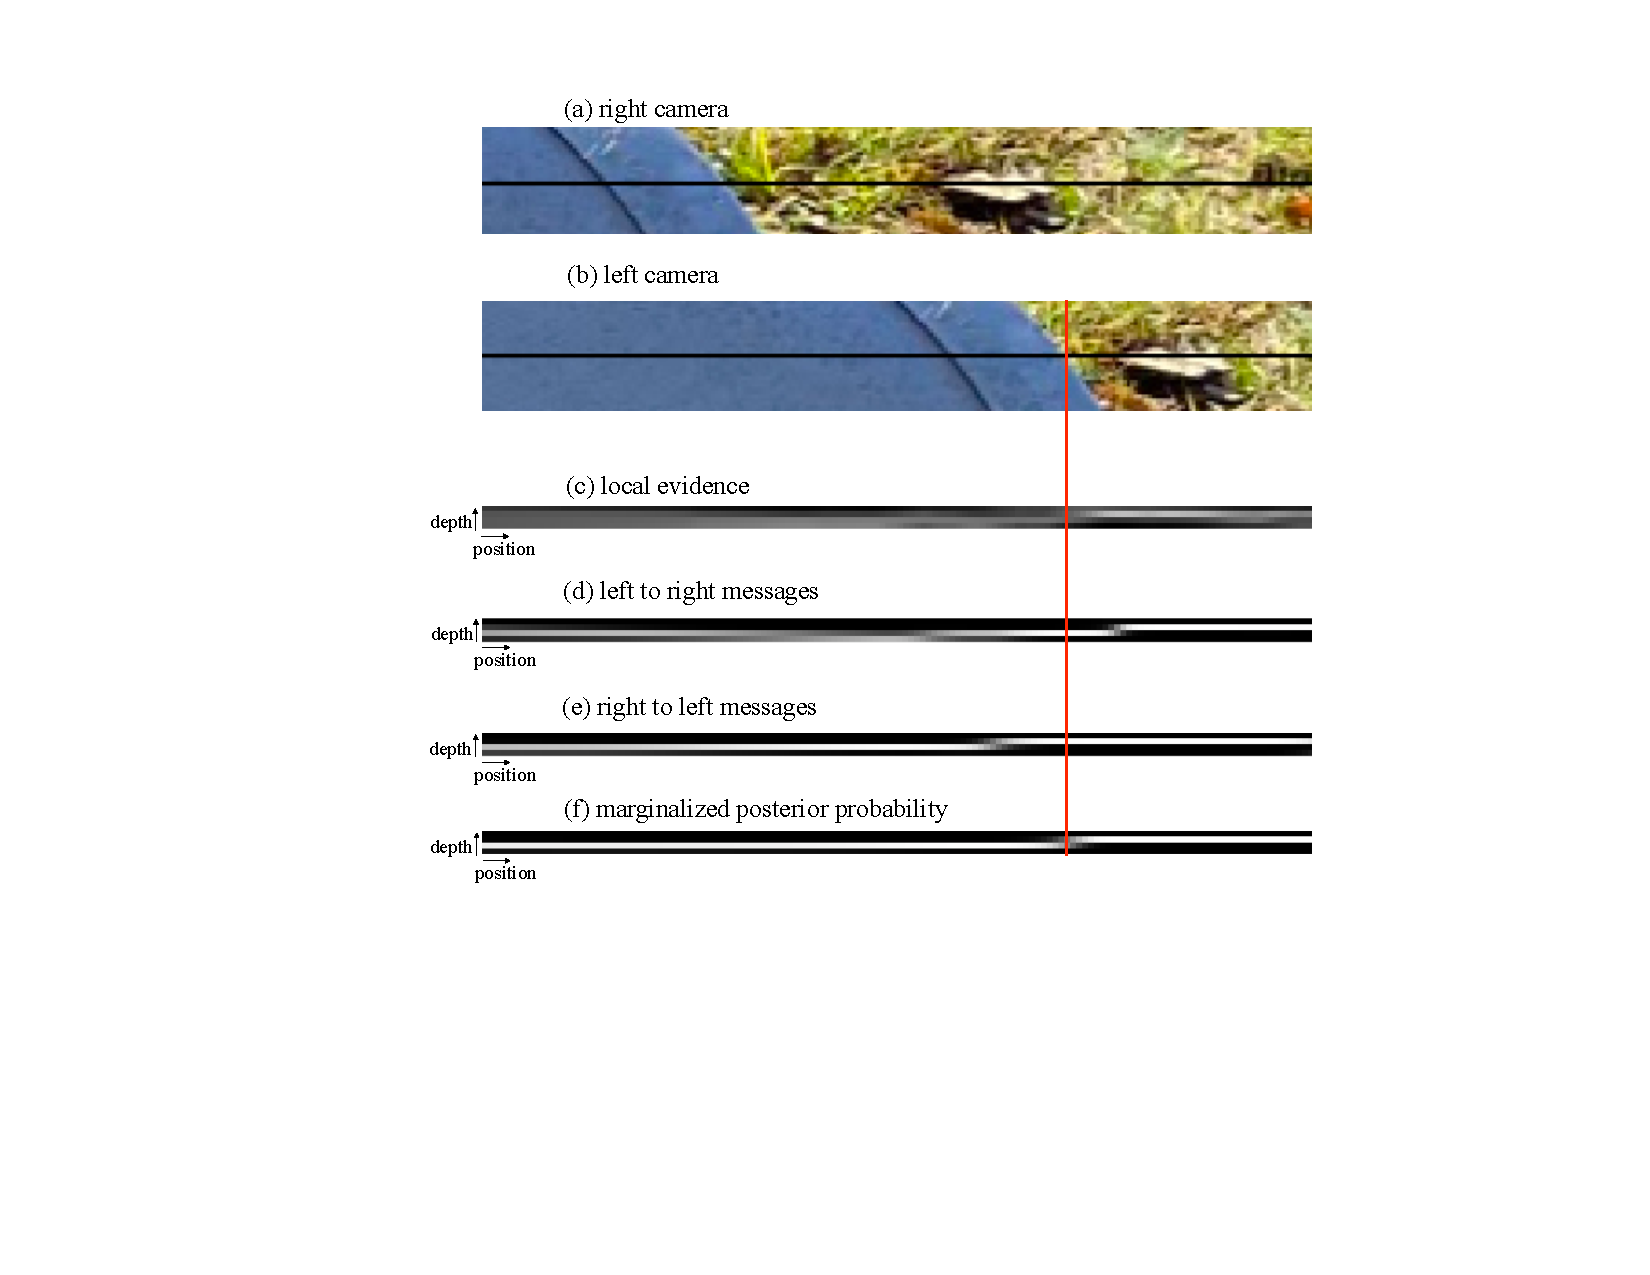
\includegraphics[width=.8\linewidth]{figures/graphical_models/bpcanoes5.pdf}
}
\caption{
Belief propagation applied to graphical model, \fig{\ref{fig:canoe3}}, for the stereo problem. (a) Right and (b) left camera views. The black line shows the analyzed row. (c) Local evidence for each depth disparity at left camera. (d) Final rightward and (e) leftward belief propagation messages at each position. (f) Final marginalized posterior probability at each left camera pixel accurately finds the depth discontinuity.}
\label{fig:canoe4}
\end{figure}


The prior probability of any configuration of pixel disparity states is described by setting the compatibility matrices, $\mathbf{\phi}[s_i, s_{i+1}]$ of the Markov chain of \fig{\ref{fig:canoe3}}.  For this example, we use a compatibility matrix referred to as the Potts Model \cite{Wu1982}:
\begin{equation}
  \mathbf{\phi}[s_i, s_{i+1}] = 
    \begin{cases}
      1, & \text{if}\ s_i = s_{i+1} \\
      \delta, & \text{otherwise}
    \end{cases}
\end{equation}
For this example, we used $\delta = 0.001$

We then ran BP (equation [\ref{eq:bpupdate}]) in a depth-first update schedule.  For this network, that involves two linear sweeps over all the nodes of the chain, first from left to right, then from right to left.  Starting from the left-most node, we updated the rightward messages one node at a time, in a rightward sweep; then, starting from the right-most node, updated all the leftward messages one node at a time, in a leftward sweep.  The results are in \fig{\ref{fig:canoe4}}(d and e), respectively.

Once all the messages were computed, we used \eqn{\ref{eq:bpmarginal}} to find the posterior marginal probability at each node. That involves, at each position, multiplying together all the incoming messages, including the local evidence.  Thus, the values shown in \fig{\ref{fig:canoe4}}{f} are the product, at each position, of \fig{\ref{fig:canoe4}}{c, d and e}.
Note that for this scanline, in this image pair, there is a depth discontinuity at location of the red vertical mark in \fig{\ref{fig:canoe4}}, namely the canoe is closer to the camera than the ground beyond the canoe that appears to the right of the canoe.  The local evidence for depth disparity, \fig{\ref{fig:canoe4}}{c}, is rather noisy, but the marginal posterior probability, after aggregating evidence along the scanline, accurately finds the depth discontinuity at the canoe boundary.

\begin{comment}
\begin{figure}
\centerline{
\sublabel{a}{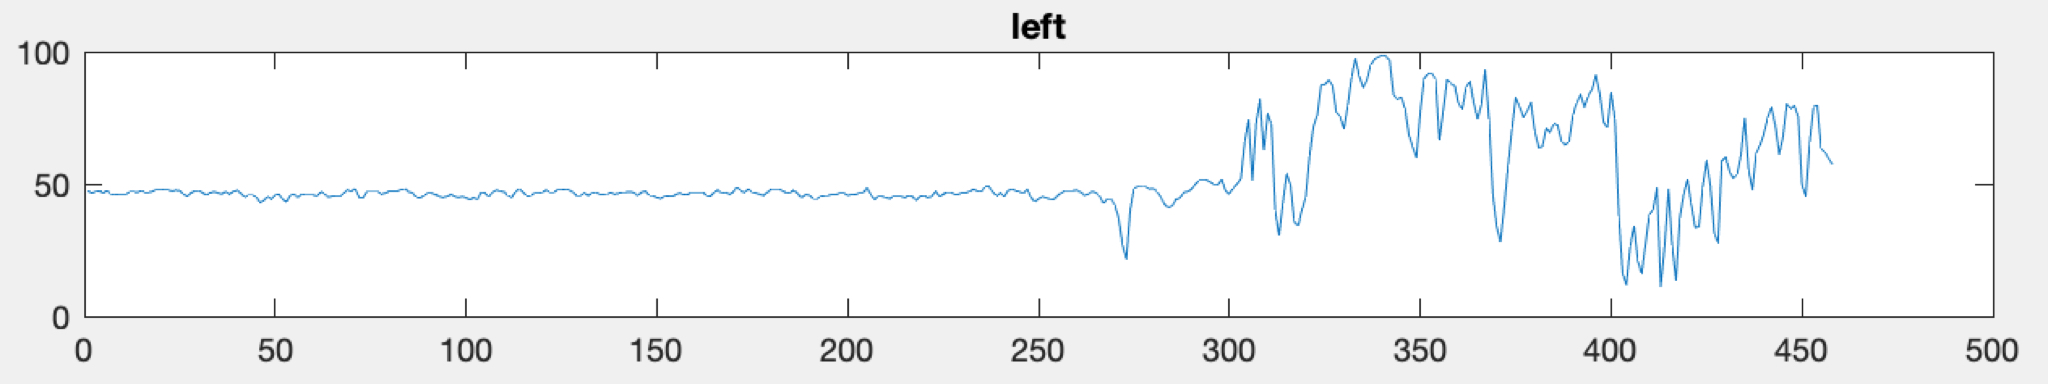
\includegraphics[width=0.80\linewidth]{figures/graphical_models/lcanoeline.jpg}}}
\centerline{
\sublabel{b}{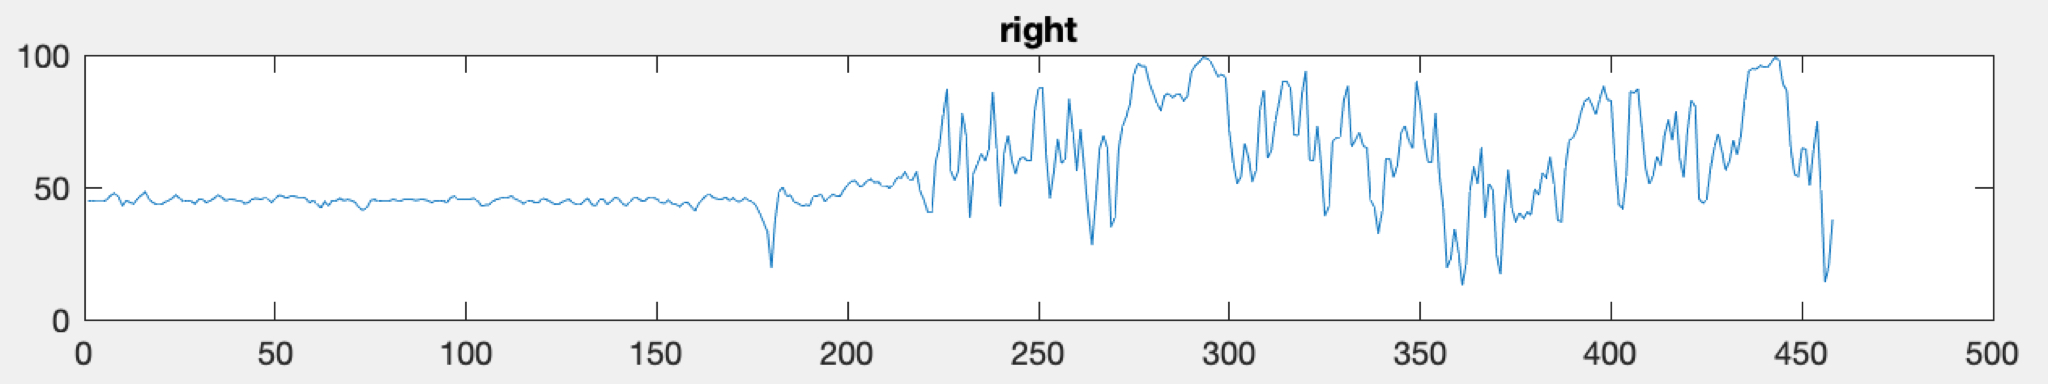
\includegraphics[width=0.80\linewidth]{figures/graphical_models/rcanoeline.jpg}}
}
\caption{(a) and (b) show the luminance traces from the scanlines marked in black in Fig.~\ref{fig:canoe1}~(c) and (d), respectively.}
\label{fig:canoe2}
\end{figure}
\end{comment}



\section{Loopy Belief Propagation}

The BP message update rules only work to give the exact marginals when
the topology of the network is that of a tree or a chain.   In general, one can show that exact
computation of marginal probabilities for graphs with loops depends on
a graph-theoretic quantity known as the {\bf treewidth} of the graph \cite{Koller2009}.  For
many graphical models of interest in vision, such as 2D Markov random
fields related to images, these quantities can be intractably large.

%But the
Message update rules are described locally, and one might imagine that
it is a useful local operation to perform, even without the global
guarantees of ordinary BP.   It turns out that is true.   Here is the algorithm, also know as
{\bf loopy belief propagation algorithm}:
\begin{enumerate}
\item Convert graph to pairwise potentials.
\item Initialize all messages to all ones, or to random values
 between 0 and 1.
\item  Run the belief propagation update rules of
  \sect{\ref{sect:bpRules}} until convergence.
\end{enumerate}

One can show that, in networks with loops, fixed points of the
belief propagation algorithm (message configurations where the
messages don't change with a message update) correspond to minima of a
well-known approximation from the statistical physics community known 
as the Bethe free energy \cite{Yedidia00b}.  In practice, the solutions found by the loopy belief propagation algorithm can be quite good \cite{Murphy1999}.
%, and other algorithms in this vein have been developed which are better still \cite{Wainwright03}.


%% \section{MAP Estimation and Energy Models}

Instead of summing over the states of other nodes, we are sometimes
interested in finding the $\mathbf{x}$ that maximizes the joint probability.  The argmax
operator passes through constant variables just as the summation sign
did.  This leads to an alternate version of the BP
algorithm, \eqn{\ref{eq:bpupdate}}, with the summation (of multiplying the vector message products by the node compatibility matrix) replaced with argmax.  This is
called the {\bf max-product} 
\index{Max-product algorithm}
version of belief propagation, and it
computes an MAP estimate of the hidden states.   
Improvements have been developed over loopy belief propagation for the
case of MAP estimation; see, for example, tree-reweighted belief propagation \cite{Kolmogorov2006} and graph cuts \cite{Zabih2004}.


\subsection{Numerical Example of Belief Propagation}
\label{sect:numerical}

Here we work though a numerical example of belief propagation.  To make the arithmetic easy,
we'll solve for the marginal probabilities in the graphical model of
two-state (0 and 1) random variables shown in \fig{\ref{fig:numerical}}.


\begin{figure}
\centerline{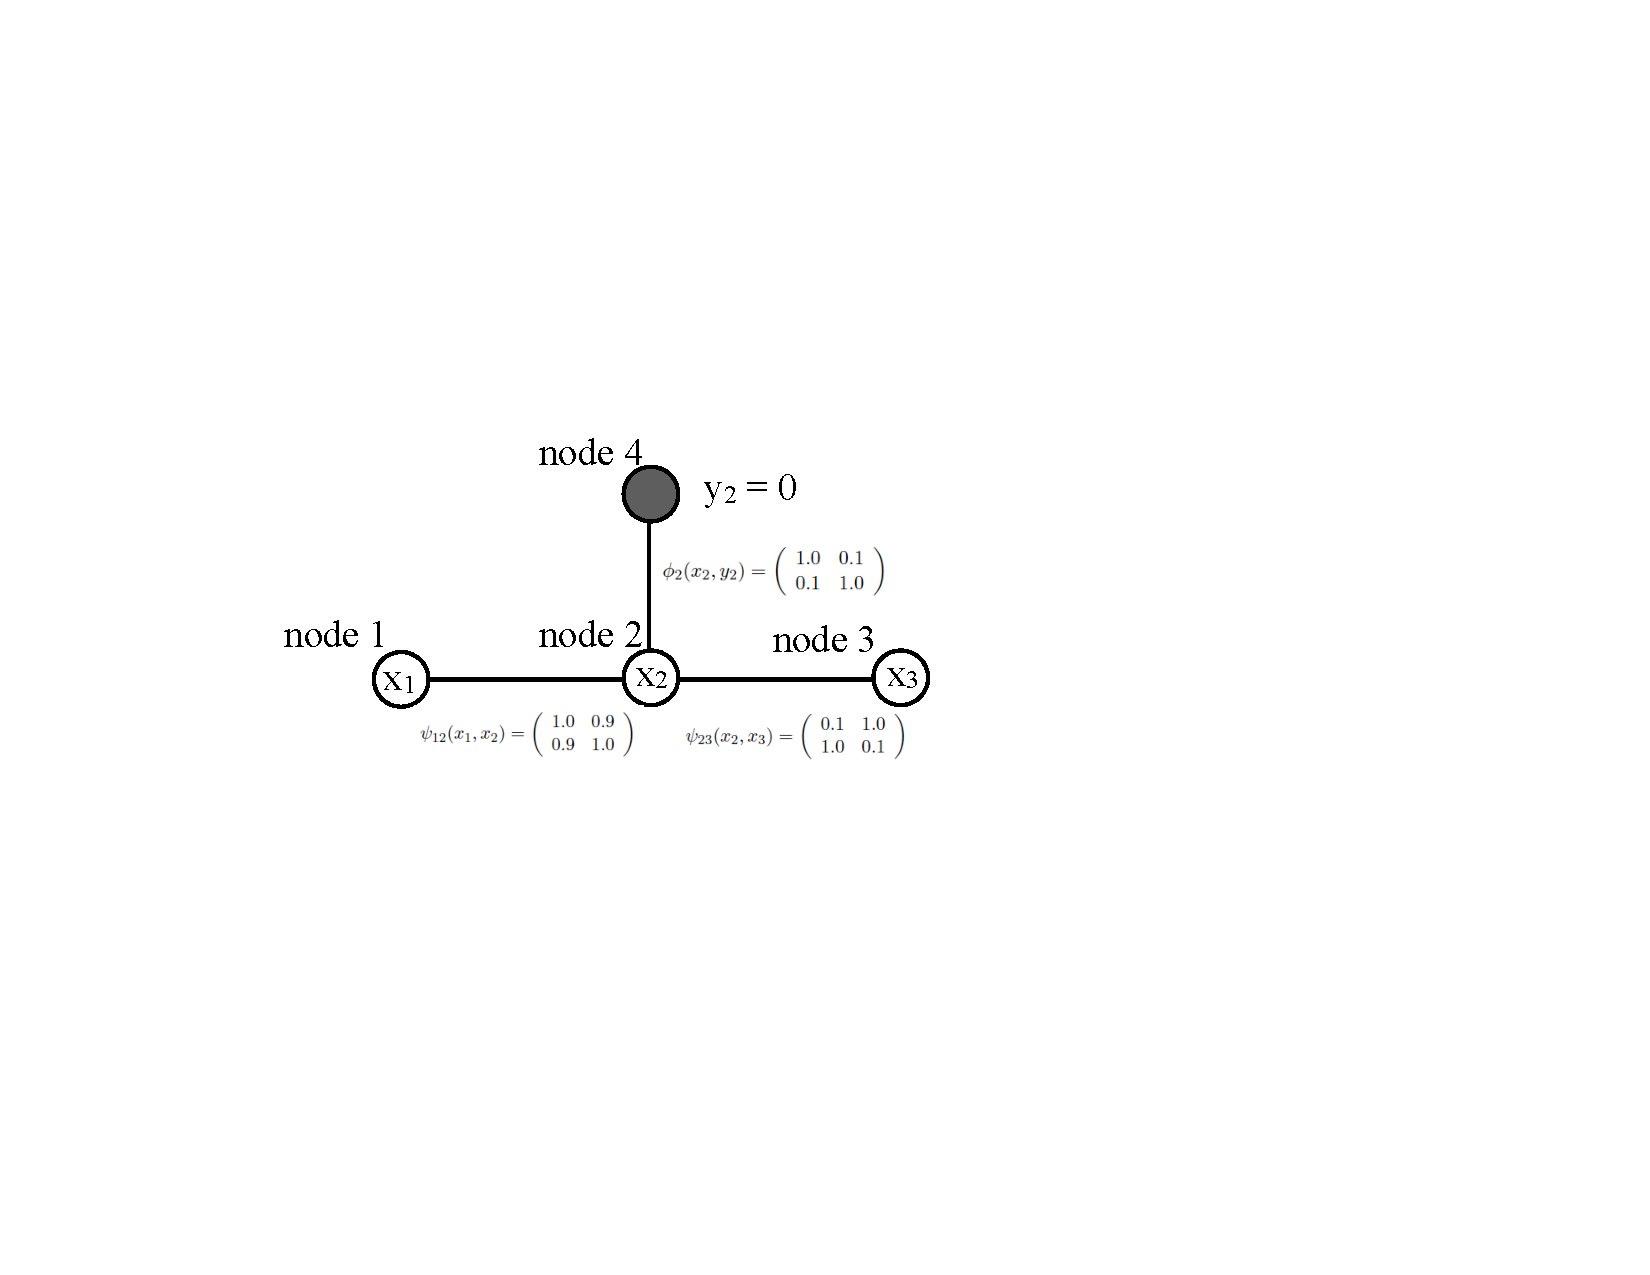
\includegraphics[width=0.48\linewidth]{figures/graphical_models/numerical2.pdf}} 
\caption{Undirected graphical model used in belief propagation example.} 
\label{fig:numerical}
\end{figure}

That
graphical model has three hidden variables, and one variable observed to
be in state 0.  The compatibility matrices are given in the arrays
below (for which the state indices are 0, then 1, reading from left to
right and top to bottom):
\begin{equation}
\psi_{12}(x_1, x_2) = 
\begin{bmatrix}
1.0 & 0.9 \\
0.9 & 1.0 
\end{bmatrix}
\end{equation}

\begin{equation}
\psi_{23}(x_2, x_3) = 
\begin{bmatrix}
0.1 & 1.0 \\
1.0 & 0.1 
\end{bmatrix}
\end{equation}

\begin{equation}
\psi_{42}(x_2, y_2) = 
\begin{bmatrix}
1.0 & 0.1 \\
0.1 & 1.0 
\end{bmatrix}
\end{equation}

Note that in defining these potential functions, we haven't taken care to normalize the joint probability, so
we'll need to normalize each marginal probability at the end
(remember $p(x_1,
x_2, x_3, y_2) = \psi_{42}(x_2, y_2) \psi_{23}(x_2, x_3) \psi_{12}(x_1,
x_2)$, which should sum to 1 after summing over all states).


For this simple toy example, we can tell what results to expect by inspection, then verify that BP is doing the right thing.  Node $x_2$ wants very much to look like $y_2=0$, because
$\psi_{42}(x_2, y_2)$ contributes a large valued to the posterior
probability when $x_2 = y_2 = 1$ or when $x_2 = y_2 = 0$.  From
$\psi_{12}(x_1, x_2) $ we see that
$x_1$ has a very mild preference to
look like $x_2$.  So we expect the marginal probability at node $x_2$
will be heavily biased toward $x_2=0$, and that node $x_1$ will have a
mild preference for state 0.  $\psi_{23}(x_2, x_3)$ encourages 
$x_3$ to be the opposite of $x_2$, so it will be biased toward the state $x_3=1$.

Let's see what belief propagation gives.  We'll
follow the parallel, synchronous update scheme for calculating
all the messages.  The leaf nodes can send messages along their
edges without waiting for any messages to be updated.  For the message
from node 1, we have
\begin{eqnarray} 
m_{12}(x_2) & = & \sum_{x_1} \psi_{12} (x_1, x_2)  \nonumber \\
& = & 
\begin{bmatrix} 
1.0 & 0.9 \\ 
0.9 & 1.0 
\end{bmatrix}
\begin{bmatrix}
1 \\ 
1
\end{bmatrix}
% \\
%& = &
=
\begin{bmatrix}
1.9 \\ 
1.9
\end{bmatrix}
%\\
%&  = &
=
k_1
\begin{bmatrix}
1 \\ 
1
\end{bmatrix}
\end{eqnarray} 
For numerical stability, we typically normalize the computed messages in \eqn{\ref{eq:bpupdate}} so
the entries sum to 1, or so their maximum entry is 1, then remember
to renormalize the final marginal probabilities to sum to 1.
Here, we will normalize the messages for simplicity, absorbing the normalization into constants, $k_i$.

The message from node 3 to node 2 is
\begin{eqnarray}
m_{32}(x_2) & = & \sum_{x_3} \psi_{32} (x_2, x_3) \nonumber  \\
& = & 
\begin{bmatrix}
0.1 & 1.0 \\
1.0 & 0.1 
\end{bmatrix}
\begin{bmatrix}
1 \\ 
1
\end{bmatrix}
% \\
%& = &
=
\begin{bmatrix}
1.1 \\
1.1
\end{bmatrix}
%\\
%&  = &
=
k_2
\begin{bmatrix}
1 \\
1
\end{bmatrix}
\end{eqnarray}

We have a nontrivial message from observed node $y_2$ (node 4) to the hidden
variable $x_2$:
\begin{eqnarray}
m_{42}(x_2) & = & \sum_{x_4} \psi_{42} (x_2, y_2)  \nonumber \\
& = & 
\begin{bmatrix}
1.0 & 0.1 \\
0.1 & 1.0 
\end{bmatrix}
\begin{bmatrix}
1 \\
0
\end{bmatrix}
%\\
%& = &
=
\begin{bmatrix}
1.0 \\
0.1
\end{bmatrix}
\end{eqnarray}
where $y_2$ has been fixed to $y_2 = 0$, thus restricting $\psi_{42}
(x_2, y_2) $ to just the first column.

Now we just have two messages left to compute before we have all
messages computed (and therefore all node marginals computed from
simple combinations of those messages).  
The message from node 2 to node 1 uses the messages from nodes 4 to 2
and 3 to 2:
\begin{eqnarray}
m_{21}(x_1) & = & \sum_{x_2} \psi_{12} (x_1, x_2)  m_{42}(x_2) m_{32}(x_2) \nonumber \\
& = & 
\begin{bmatrix}
1.0 & 0.9 \\
0.9 & 1.0 
\end{bmatrix}
\left(
\begin{bmatrix}
1.0 \\
0.1
\end{bmatrix}
\hadamard
\begin{bmatrix}
1 \\
1
\end{bmatrix}
\right)
=
\begin{bmatrix}
1.09 \\
1.0
\end{bmatrix}
\end{eqnarray}

The final message is that from node 2 to node 3 (since $y_2$ is
observed, we don't need to compute the message from node 2 to node
4).  That message is:
\begin{eqnarray}
m_{23}(x_3) & = & \sum_{x_2} \psi_{23} (x_2, x_3)   m_{42}(x_2) m_{12}(x_2) \nonumber  \\
& = & 
\begin{bmatrix}
0.1 & 1.0 \\
1.0 & 0.1 
\end{bmatrix}
\left(
\begin{bmatrix}
1.0 \\
0.1
\end{bmatrix}
\hadamard
\begin{bmatrix}
1 \\
1
\end{bmatrix}
\right) 
=
\begin{bmatrix}
0.2 \\
1.01
\end{bmatrix}
\end{eqnarray}

Now that we've computed all the messages, let's look at the marginals
of the three hidden nodes.  The product of all the messages arriving
at node 1 is just the one message, $m_{21}(x_1)$, so we have
(introducing constant $k_3$ to normalize the product of messages to be a
probability distribution)
\begin{equation}
p_1(x_1) = k m_{21}(x_1) 
=
\frac{1}{2.09}
\begin{bmatrix}
1.09 \\
1.0
\end{bmatrix}
\end{equation}
As we knew it should, node 1 shows a slight preference for state 0.

The marginal at node 2 is proportional to the product of three messages.
Two of those are trivial messages, but we'll show them all for
completeness:
\begin{eqnarray}
p_2(x_2) & = & k_4 m_{12}(x_2)  m_{42}(x_2)  m_{32}(x_2) \\
& = & k_4 
\begin{bmatrix} 
1 \\ 
1
\end{bmatrix}
\hadamard
\begin{bmatrix}
1.0 \\
0.1
\end{bmatrix}
\hadamard
\begin{bmatrix}
1 \\ 
1
\end{bmatrix}
%\\
%& = &
=
\frac{1}{1.1}
\begin{bmatrix}
1.0 \\
0.1
\end{bmatrix}
\end{eqnarray}
As expected, belief propagation reveals a strong bias for node 2 being in state 0.

Finally, for the marginal probability at node 3, we have
\begin{equation}
p_3(x_3) = k_5 m_{23}(x_3) 
=
\frac{1}{1.21}
\begin{bmatrix}
0.2 \\
1.01
\end{bmatrix}
\end{equation}
As predicted, this variable is biased toward being in state 1.

By running belief propagation within this tree, we have computed the
exact marginal probabilities at each node, reusing the intermediate
sums across different marginalizations, and exploiting the structure
of the joint probability to perform the computation efficiently.  If
nothing were known about the joint probability structure, the
marginalization cost would grow exponentially with the number of nodes
in the network.  But if the graph structure corresponding to the joint
probability is known to be a chain or a tree, then the marginalization
cost only grows linearly with the number of nodes, and is quadratic in
the node state dimensions.  The belief propagation algorithm enables inference in many large-scale problems.

\section{Relationship of Probabilistic Graphical Models to Neural Networks}

The probabilistic graphical models (PGMs) we studied in this chapter and neural networks (NNs) share some characteristics, but are quite different.  Both share a graph structure, with nodes and edges, but the nodes and edges mean different things in each case.  Below is a brief summary of the differences:

\begin{itemize}
    \item {\bf Nodes}: The nodes of a NN diagram typically represent a real-valued scalar activations.  The nodes of a PGM represent a random variable, real or discrete-valued, and scalars or vectors.
    \item {\bf Edges}:  Edges in PGMs determine statistical dependencies.  Edges in NNs determine which are involved in a linear summation to the next layer.
    \item {\bf Computation}:  The big difference between PGMs and NNs lies in what they calculate.  PGMs represent factorized probability distributions and pass messages that allow for the computation of  probabilities, for example, the marginal probability at a node. In contrast, NNs compute results that minimize some expected loss or an energy function \cite{LeCun2006,LeCun2007}.  That different goal, that is, minimizing an expected loss rather than calculating a probability, allows for more general computations by a neural network at the cost of output that may be less modular or less interpretable because they are not probabilities.
\end{itemize}
Both PGMs and NNs can have nodes organized into grid-like structures but also more generally in arbitrary graphs; see, for example, \cite{Gilmer2017,Kipf2017}.

\section{Concluding Remarks}

Probabilistic graphical models provide a modular representation for complex joint probability distributions. Nodes can represent pixels, scenes, objects, or object parts, while the edges describe the conditional independence structure. For tree-like graphs, belief propagation delivers optimal inference. In general graphs with loops, it can give a reasonable approximation.
